% DualHash Beamer slides
% Visual style: aligned with mossp_slides.tex (Boadilla + infolines, mathserif, 9pt)
% Content source: SIIM paper (main.tex + sections/ + ex_shared.tex)

\documentclass[mathserif,compress,override,9pt]{beamer}
\usepackage{beamerthemesplit}
\usepackage{cases}
\usepackage[english]{babel}

\usepackage{graphicx,subfigure}
\usepackage{hyperref}
\usepackage{amsfonts}
\usepackage[round,authoryear]{natbib}
\usepackage{amsmath,amssymb,amsthm,amscd,amsxtra}
\usepackage{bm}
\usepackage{multirow}
\usepackage{booktabs}
\usepackage{enumerate}
\usepackage{textcomp}
\usepackage{color,xcolor}
\usepackage{manfnt}
\usepackage{tikz}
\usetikzlibrary{arrows.meta}
\usepackage{framed}
\usepackage{algorithm}
\usepackage{algorithmic,float}
\usepackage{amsopn}
\usepackage{makecell}
\usepackage{diagbox}
\graphicspath{{./}{../}{slides/}{paper/}{../paper/}}

\usetheme{Boadilla}
\useoutertheme{infolines}
\setbeamertemplate{itemize item}{{\color{blue}$\blacktriangleright$}}
\setbeamertemplate{itemize subitem}{{\color{blue}$\blacktriangleright$}}
\setbeamertemplate{itemize subsubitem}{{\color{blue}$\blacktriangleright$}}

\setbeamertemplate{caption}[numbered]
\setbeamertemplate{theorems}[numbered]
\numberwithin{equation}{section}

\setbeamertemplate{navigation symbols}{}
\makeatletter
\setbeamertemplate{section in toc}{%
  \leavevmode
  \leftskip=1.5em
  \llap{\@Roman{\inserttocsectionnumber}.\hskip0.6em}%
  \inserttocsection\par
}
\makeatother

% Macros (merged from mossp_slides.tex and ex_shared.tex)
\newcommand{\nii}{\noindent}
\newcommand{\nn}{\nonumber}
\newcommand{\RR}{\mathbb{R}}
\newcommand{\EE}{\mathbb{E}}
\newcommand{\zero}{\bm{0}}
\newcommand{\One}{\bm{1}}
\newcommand{\prox}{\mathrm{prox}}
\newcommand{\dist}{\operatorname{dist}}
\newcommand{\tf}{\mathbf{f}}
\newcommand{\bx}{\bm{x}}
\newcommand{\bb}{\bm{b}}
\newcommand{\bc}{\bm{c}}
\newcommand{\ba}{\bm{a}}
\newcommand{\bd}{\bm{d}}
\newcommand{\be}{\bm{e}}
\newcommand{\bs}{\bm{s}}
\newcommand{\bu}{\bm{u}}
\newcommand{\bv}{\bm{v}}
\newcommand{\bw}{\bm{w}}
\newcommand{\by}{\bm{y}}
\newcommand{\bz}{\bm{z}}
\newcommand{\bg}{\bm{g}}
\newcommand{\bp}{\bm{p}}
\newcommand{\bxi}{\bm{\xi}}
\newcommand{\blambda}{\bm{\lambda}}
\newcommand{\bA}{\bm{A}}
\newcommand{\bD}{\bm{D}}
\newcommand{\bS}{\bm{S}}
\newcommand{\bW}{\bm{W}}
\newcommand{\bX}{\bm{X}}
\newcommand{\bY}{\bm{Y}}
\newcommand{\bB}{\bm{B}}
\newcommand{\bC}{\bm{C}}
\newcommand{\bG}{\bm{G}}
\newcommand{\bLmbd}{\bm{\Lambda}}
\newcommand{\bM}{\bm{M}}
\newcommand{\calB}{\mathcal{B}}
\newcommand{\calL}{\mathcal{L}}
\newcommand{\calO}{\mathcal{O}}
\newcommand{\calJ}{\mathcal{J}}
\newcommand{\calQ}{\mathcal{Q}}
\newcommand{\dom}{\mathrm{dom}}
\newcommand{\interior}{\mathrm{int}}
\newcommand{\ran}{\mathrm{ran}}
\newcommand{\Id}{\mathrm{Id}}
\newcommand\argmax{\mathop{\mathrm{argmax}}}
\newcommand\argmin{\mathop{\mathrm{argmin}}}
\newcommand{\blue}[1]{\textcolor{blue}{#1}}
\newcommand{\red}[1]{\textcolor{red}{#1}}
\def\st{\hbox{s.t.}}
\def\ds{\displaystyle}
\providecommand{\foo}{\footnotesize}
\newcommand{\mathhl}[2]{%
  \begingroup
  \setlength{\fboxsep}{1.5pt}%
  \colorbox{#1}{$\displaystyle\mathstrut #2$}%
  \endgroup
}
\definecolor{dualgreen}{RGB}{218,247,217}
\definecolor{dualpurple}{RGB}{232,226,255}
\makeatletter
\colorlet{beamerblue}{beamer@blendedblue}
\makeatother

\addtobeamertemplate{frametitle}{}{%
  \begin{tikzpicture}[remember picture,overlay]
    \node[anchor=north east,xshift=-0.24cm,yshift=-0.14cm]
      at (current page.north east)
      {
\includegraphics[height=0.95cm]{figures/single-logo.pdf}};
  \end{tikzpicture}%
}

\renewcommand{\algorithmicrequire}{\textbf{Input:}}
\renewcommand{\algorithmicensure}{\textbf{Output:}}

\theoremstyle{remark}
\newtheorem*{remark}{Remark}

\setbeamertemplate{footline}{%
  \leavevmode%
  \hbox{%
    \begin{beamercolorbox}[wd=.17\paperwidth,ht=2.25ex,dp=1ex,center]{author in head/foot}%
      \usebeamerfont{author in head/foot}\insertshortauthor~(\insertshortinstitute)
    \end{beamercolorbox}%
    \begin{beamercolorbox}[wd=.60\paperwidth,ht=2.25ex,dp=1ex,center]{title in head/foot}%
      \usebeamerfont{title in head/foot}\insertshorttitle
    \end{beamercolorbox}%
    \begin{beamercolorbox}[wd=.23\paperwidth,ht=2.25ex,dp=1ex,right]{date in head/foot}%
      \usebeamerfont{date in head/foot}\insertshortdate{}\hspace*{2em}\insertframenumber{} / \inserttotalframenumber\hspace*{1ex}
    \end{beamercolorbox}%
  }%
  \vskip0pt%
}

\AtBeginSection[]{%
  \begin{frame}[plain]
    \centering
    \vfill
    {\usebeamerfont{title}\color{beamerblue}\Large\Roman{section}. \insertsectionhead}
    \vfill
  \end{frame}
}

\title[DUALHASH: A STOCHASTIC PRIMAL-DUAL ALGORITHM]{DualHash: A Stochastic Primal-Dual Algorithm\\
with Theoretical Guarantee for Deep Hashing}
\author[C. Cui]{\large Chunfeng Cui, Beihang University\\[0.4em]
 {\small Joint work with Luxuan Li and Prof. Xiao Wang}}
\institute[BUAA]{{\normalsize @ Nanjing University}}
\date[Auguest 22, 2026]{Auguest 22, 2026}

\begin{document}

\frame{\titlepage}


\begin{frame}{Outline}
\tableofcontents
\end{frame}


\section{Background and Modeling}

% ========== Page 1: What ==========
\begin{frame}[t]{Deep Hashing: From Images to Binary Codes}
\small
\vspace{0.05cm}

\begin{columns}[T,onlytextwidth]
  \column{0.48\textwidth}
  {\color{beamerblue}\textbf{Learning to Hash}}
  \vspace{0.06cm}

\begin{center}
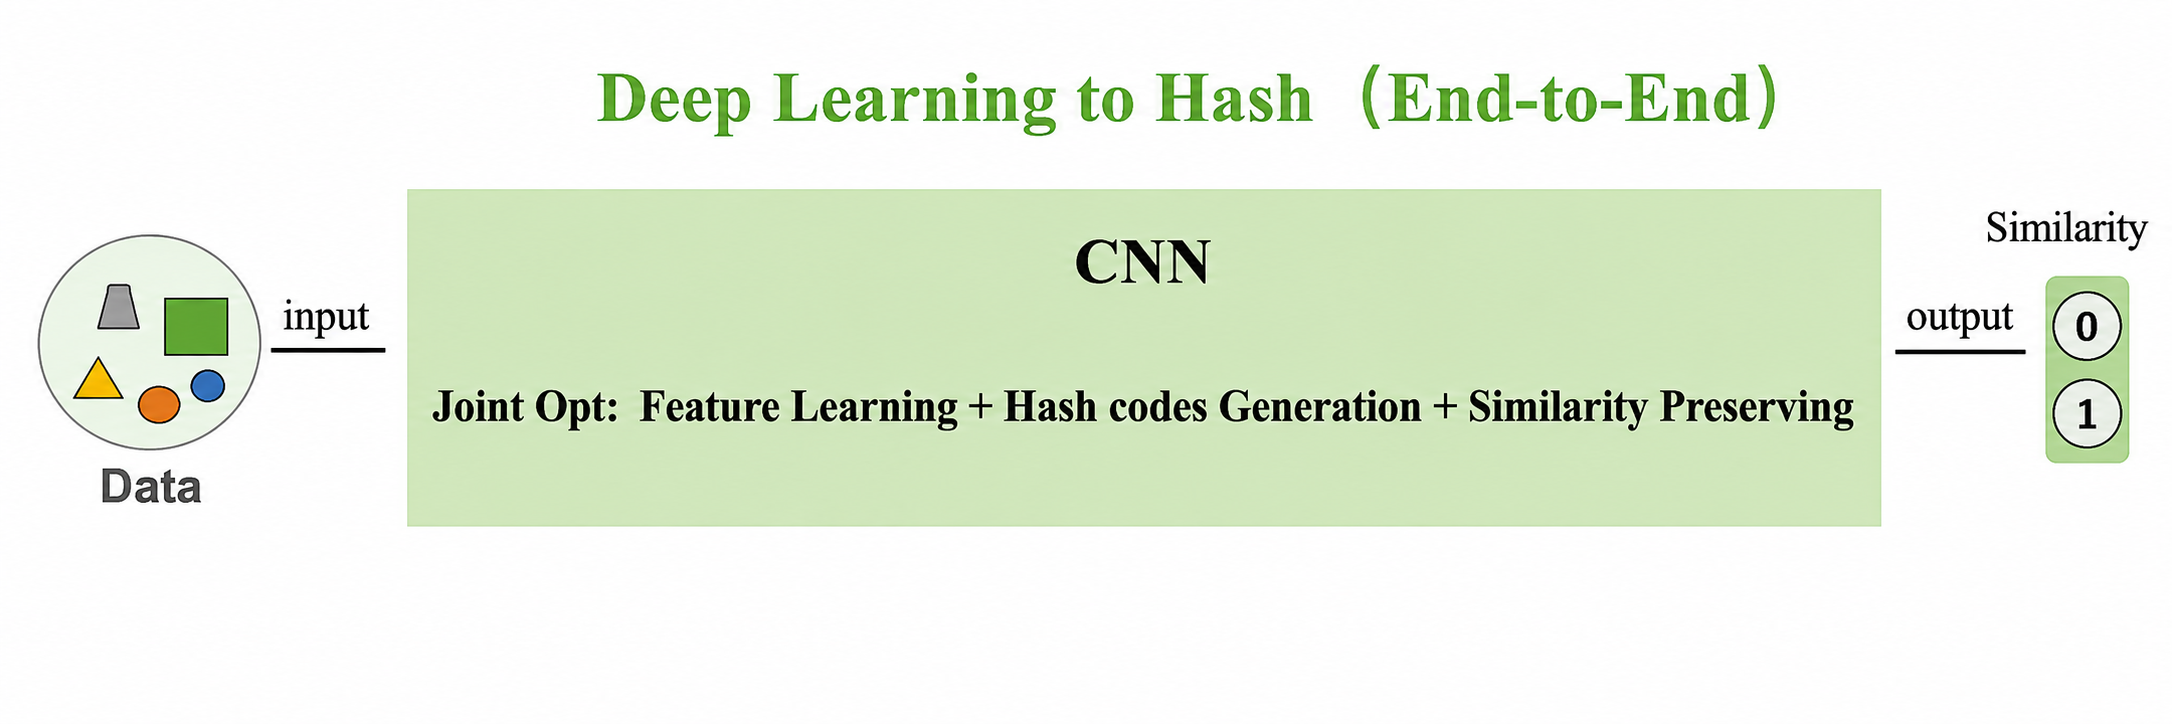
\includegraphics[width=0.9\textwidth,height=0.4\textheight,keepaspectratio]{figures/rc1/d2h.png}
\end{center}
\begin{itemize}
  % \setlength{\itemsep}{0.16cm}
  \item \textbf{Challenge: Scalable Retrieval} \\
        Large-scale image retrieval demands fast similarity search
        over millions of items.
  \item \textbf{Hashing: Compact Binary Codes} \\
        Encoding images as $\pm 1$ binary codes enables efficient
        Hamming-distance comparison with up to $512\times$ storage compression.
  \item \textbf{Deep Hashing: Learned Semantics} \\
        Neural networks learn hash projections that preserve
        semantic neighborhood structures.
\end{itemize}
  \column{0.49\textwidth}
  \centering
  \vspace{0.5cm}
  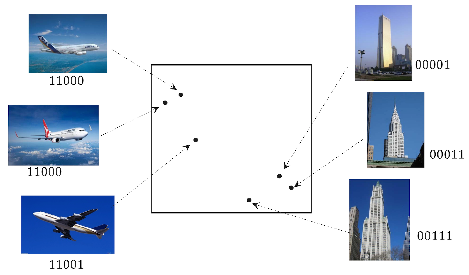
\includegraphics[width=1\linewidth,height=4cm,keepaspectratio]{figures/rc1/l2h.png}
\end{columns}

\vspace{-0.06cm}

\end{frame}



\begin{frame}[t]{Mathematical Formulation in Deep Hashing}
\small
\vspace{0.06cm}

\[
\min_{\bx\in\RR^{d_{\bx}}}\
\frac{1}{n}\sum_{i=1}^{n}
\ell_{s,i}\bigl(\red{\operatorname{sgn}}(\bC_i(\bx))\bigr).
\]

\vspace{-0.06cm}
\begin{itemize}
  % \setlength{\itemsep}{0.08cm}
  \item $\bx\in\RR^{d_{\bx}}$ denotes the trainable neural network parameters.
  \item $\bC_i(\bx)\in\RR^d$ denotes the output for the $i$-th sample.
  \item $\operatorname{sgn}(\bC_i(\bx))\in\{-1,+1\}^d$ denotes the binary hash code.
\end{itemize}

\vspace{0.06cm}
\begin{block}{Quantization Difficulties}
\small
\begin{itemize}
% \setlength{\itemsep}{0.08cm}
\item[$\triangleright$] \red{Zero gradient:}
\[
sgn(100)-sgn(0.1)/100-0.1 = 0
\]
      $\operatorname{sgn}(\cdot)$ has zero
      gradient almost everywhere and makes gradient-based optimization methods ineffective.
\item[$\triangleright$] 
% 
% \red{Quantization error:}
      $\operatorname{sgn}(\cdot)$ renders outputs of vastly different
      magnitudes indistinguishable.
\end{itemize}
\end{block}

\vspace{-0.04cm}
% \begin{center}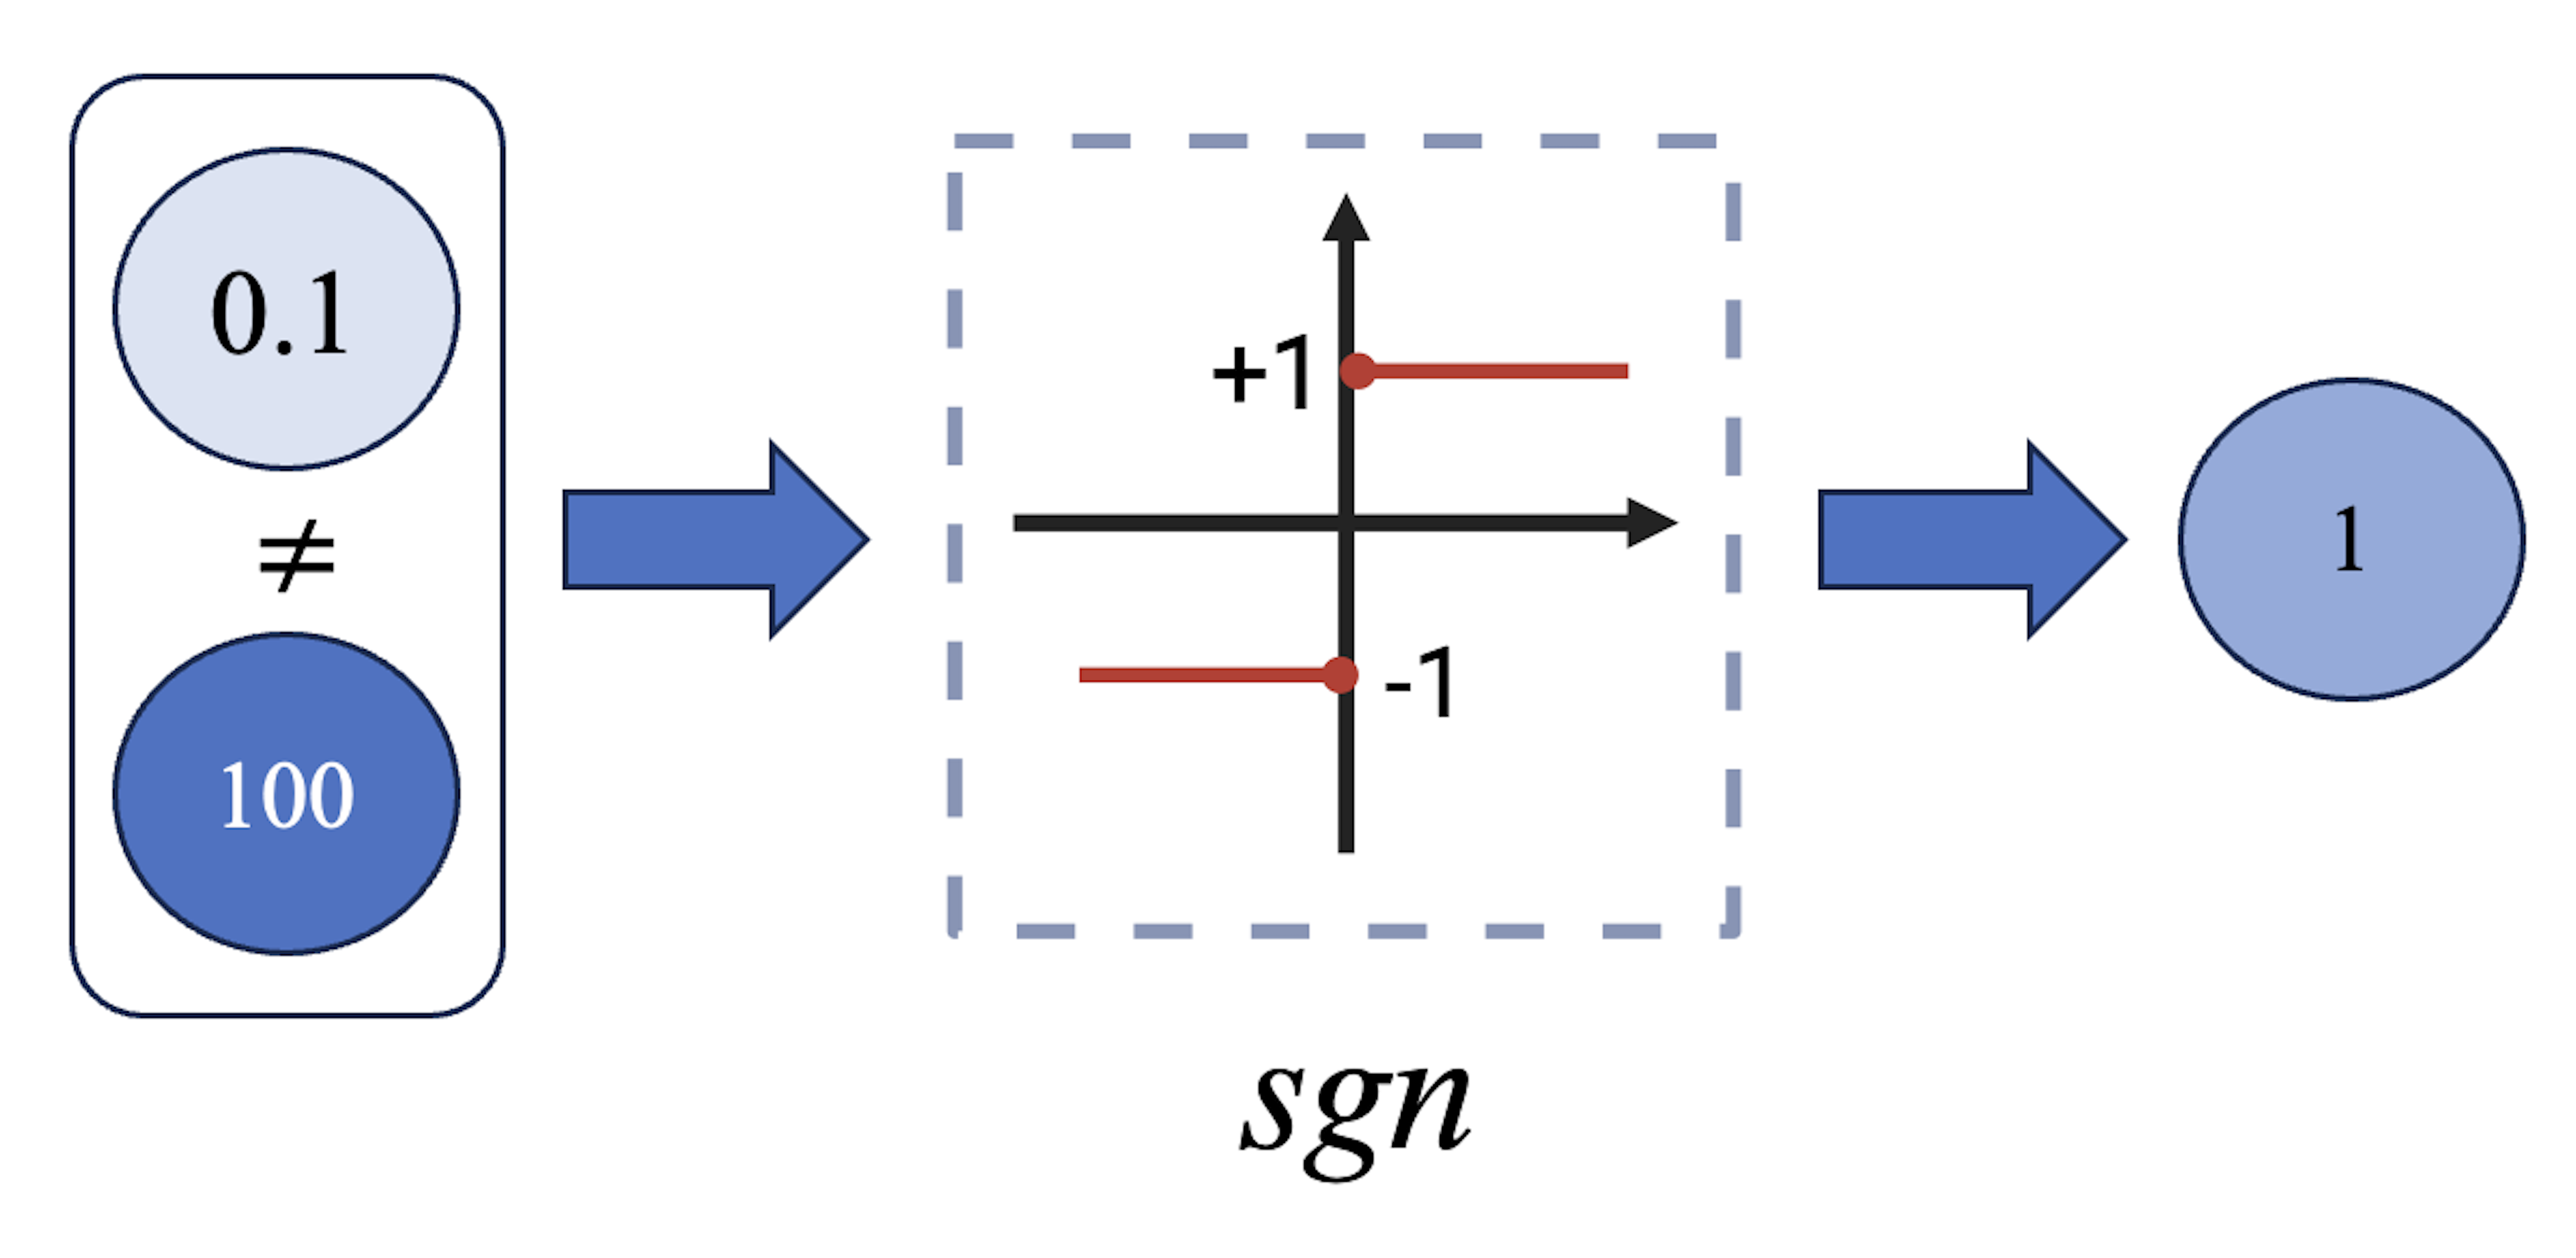
\includegraphics[width=0.72\textwidth,height=0.25\textheight,keepaspectratio]{papers_img/quantization_error_cha.png}
% \end{center}

\end{frame}


\begin{frame}[t]{Solution: From Discrete Model to Continuous Optimization}
\small

\vspace{0.2cm}

\begin{columns}[T,onlytextwidth]
  \begin{column}{0.60\textwidth}
  \vspace{0.2cm}
  \begin{itemize}
    % \setlength{\itemsep}{0.07cm}
    \item[$\triangleright$] \textbf{Continuous relaxation:}
    replace $\operatorname{sgn}(\bC_i(\bx))$ by a continuous network
    output $\bD_i(\bx)$ during training.
    \item[$\triangleright$] \textbf{Quantization regularization:} introduce W-type regularization
    \[
      h(\bz)=\lambda_h\bigl\||\bz|-\One\bigr\|_1,\qquad \lambda_h>0
    \]
    to drive continuous outputs toward $\{-1,+1\}^d$.
  \end{itemize}
  \end{column}

  \begin{column}{0.38\textwidth}
  \centering
  \vspace{0.1cm}
  \begin{tikzpicture}[x=0.72cm,y=0.94cm,>=Stealth,line cap=round,line join=round]
        \draw[-{Stealth},thin] (-2.9,0) -- (2.9,0) node[below right] {$b$};
        \draw[-{Stealth},thin] (0,-0.7) -- (0,2.9);
        \draw[line width=1.0pt] (-2.6,1.9) -- (-1,0) -- (0,2.1) -- (1,0) -- (2.6,1.9);
        \node at (-1,-0.42) {$-1$};
        \node at (1,-0.42) {$+1$};
        \node at (0,-1.15) {W-type regularizer $h(z)$};
  \end{tikzpicture}

  % \vspace{0.15cm}
  % {\scriptsize W-type: nonconvex, drives variables toward $\pm 1$, \blue{less biased} for binary codes than the convex $\ell_1$ norm.}
  \end{column}
\end{columns}
\end{frame}

\begin{frame}{}
\vspace{0.08cm}
% 加一个pass 
\[
\min_{\bx\in\RR^{d_{\bx}}}\
\frac{1}{n}\sum_{i=1}^{n}
\ell_{s,i}\bigl(\red{\operatorname{sgn}}(\bC_i(\bx))\bigr).
\]

% 加一个箭头

Our goal: Optimization the  W-type regularized problem efficiently? 

\[
\min_{\bx\in\RR^{d_{\bx}}}\quad
\frac{1}{n}\sum_{i=1}^n f_i(\bx)
+\sum_{i=1}^n h(\bD_i(\bx)).
\]

\vspace{0.10cm}
\begin{itemize}
  % \setlength{\itemsep}{0.05cm}
  \item Finite-sum optimization: $n$ can be large.
  \item $f_i(\bx)=\ell_{s,i}(\bx)+\frac{\mu}{2}\|\bx\|^2$ and
        $\bD_i(\bx)$ are continuously differentiable.
  \item $h$ is a proper l.s.c. nonconvex regularizer.
\end{itemize}

    
\end{frame}
\begin{frame}[t]{The Nonsmooth Composite in Deep Hashing}
\vspace{-0.2cm}

\begin{center}
  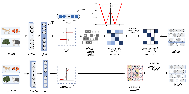
\includegraphics[width=0.97\textwidth,height=0.60\textheight,keepaspectratio]{papers_img/comparision_D2H_final.pdf}
\end{center}

\vspace{0.2cm}
\begin{itemize}
% \setlength{\itemsep}{0.08cm}
  \item Regularization acts on the network output, so the nonsmooth
composite $h(\bD_i(\bx))$ needs to be handled explicitly.
  \item \red{New challenges emerge in optimization}.
\end{itemize}

\end{frame}

\begin{frame}{Related Work: Optimization in Deep Hashing}
\vfill
{\footnotesize
\begin{center}
\setlength{\tabcolsep}{2pt}
\renewcommand{\arraystretch}{1.10}
% Original table retained for reference.
% \begin{tabular}{cccccc}
% \toprule
% \textbf{Type}\textsuperscript{*}
% & \textbf{Method}
% & \textbf{Model}\textsuperscript{\(\dagger\)}
% & \textbf{Quant. Loss}
% & \textbf{Optimization}\textsuperscript{\(\S\)}
% & \textbf{Complexity}\textsuperscript{\(\P\)} \\
% \midrule
% \multirow{3}{*}{Discrete}
% & DDSH~[4] & $ \ell_s(\bb) + Q(\bu, \bb)$ & $\|\cdot\|^2$ & BQP & \multirow{10}{*}{\red{---}} \\
% & DSDH~[17] & \multirow{2}{*}{$ \ell_s(\bu) + Q(\bu, \bb)$} & \multirow{2}{*}{$\|\cdot\|^2$} & $\operatorname{sgn}$ update & \\
% & DPSH~[18] & & & DCC & \\
% \cmidrule(lr){1-5}
% \multirow{6}{*}{Continuous}
% & DCH~[19] & \multirow{4}{*}{$ \ell_s(\bu) + h(\bu)$} & $\log(1+\frac{\operatorname{dist}_{h}(|\bu|,\mathbf1)}{\gamma})$ & \multirow{4}{*}{SGDM} & \\
% & DNNH~[20] & & $\mathcal{I}_{[-1,1]^d}$ & & \\
% & DSH~[2] & & $\bigl||\bu|-\One\bigr|_1$ & & \\
% & DTSH~[13] & & $\bigl||\bu|-\One\bigr|_2^2$ & & \\
% \cmidrule(lr){2-5}
% & HashNet~[3] & $ \ell_s(\bu)$ & --- & SGDM & \\
% & OrthoHash~[15] & $ \ell_s(\bu)$ & --- & Adam & \\
% \bottomrule
% \end{tabular}
{
\[
  \red{\min_{\bx}\ F(\bx):} =f(\bx)+h(\bD(\bx)),
  \qquad
  f(\bx)=\frac{1}{n}\sum_{i=1}^{n}f_i(\bx)
\]
}
% u_i = sgn(bi); 
\begin{tabular}{cccccc}
\toprule
\textbf{Type}\textsuperscript{*}
& \textbf{Method}
& \textbf{Model}\textsuperscript{\(\dagger\)}
& \textbf{Quant. Loss}
& \textbf{Optimization}\textsuperscript{\(\S\)}
& \textbf{Complexity}\textsuperscript{\(\P\)} \\
\midrule
\multirow{3}{*}{Discrete}
& DDSH~\blue{[JCL18]} & $ \ell_s(\bb) + Q(\bu, \bb)$ & $\|\cdot\|^2$ & BQP & \multirow{10}{*}{\red{---}} \\
& DSDH~\blue{[LSHT17]} & \multirow{2}{*}{$ \ell_s(\bu) + Q(\bu, \bb)$} & \multirow{2}{*}{$\|\cdot\|^2$} & $\operatorname{sgn}$ update & \\
& DPSH~\blue{[LWK16]} & & & DCC & \\
\cmidrule(lr){1-5}
\multirow{6}{*}{Continuous}
& DCH~\blue{[CLLW18]} & \multirow{4}{*}{$ \ell_s(\bu) + h(\bu)$} & $\log(1+\frac{\operatorname{dist}_{h}(|\bu|,\mathbf1)}{\gamma})$ & \multirow{4}{*}{SGDM} & \\
& DNNH~\blue{[LPLY15]} & & $\mathcal{I}_{[-1,1]^d}$ & & \\
& DSH~\blue{[LWSC16]} & & $\bigl||\bu|-\One\bigr|_1$ & & \\
& DTSH~\blue{[WSK16]} & & $\bigl||\bu|-\One\bigr|_2^2$ & & \\
\cmidrule(lr){2-5}
& HashNet~\blue{[CLWY17]} & $ \ell_s(\bu)$ & --- & SGDM & \\
& OrthoHash~\blue{[HNZCSX21]} & $ \ell_s(\bu)$ & --- & Adam & \\
\bottomrule
\end{tabular}
\end{center}
\vspace{0.08cm}
\textsuperscript{*}Discrete methods explicitly update binary codes \(\bb\); continuous methods optimize network outputs \(\bu=\bD_i(\bx)\).
\textsuperscript{\(\dagger\)}\(\ell_s\): similarity loss; \(Q\) or \(h\): quantization penalty.
\textsuperscript{\(\S\)}SGDM: SGD with momentum.
\textsuperscript{\(\P\)}---: no reported non-asymptotic complexity guarantee.
}
\vfill
\end{frame}

\begin{frame}[t]{Related Work: Nonsmooth Composite Optimization}
\small
\vspace{-0.3cm}


\vspace{-0.05cm}

{\footnotesize
\[
  \bD(\bx):=(\bD_1(\bx),\dots,\bD_n(\bx)) \text{ is nonconvex},\quad
  h:\text{nonconvex, nonsmooth}.
\]
}
\vspace{-0.24cm}
\begin{itemize}
% \setlength{\itemsep}{0.05cm}

\item[\blue{$\bullet$}] \textbf{Stochastic First-Order / Proximal Gradient Methods}\\[-0.02cm]
{\scriptsize [Liu et al., 2016; Cao et al., 2017; Jiang et al., 2018; Bai et al., 2019]}
\vspace{-0.04cm}
\begin{itemize}
  \setlength{\itemsep}{0.02cm}
  % \item Deep hashing methods typically employ optimizers such as SGD and Adam,
  %     with \red{limited} convergence analysis for the \red{nonconvex nonsmooth} case
  % \vspace{-0.14cm}
  % {\scriptsize
  % \[
  %   \bx^{k+1}=\bx^k-\eta_k {\bg^k},
  %   \qquad
  %   {\bg^k}\in\partial F(\bx^k;\xi_k).
  % \]
  % }
  % \vspace{-0.4cm}
  \item Stochastic proximal methods require computing
  \(\red{\prox_{h\circ \bD}}\), but this proximal operator is
  \red{generally unavailable}.
\end{itemize}

\item[\blue{$\bullet$}] \textbf{Nonlinear Composite Optimization Methods}\\[-0.02cm]
{\scriptsize [Davis and Drusvyatskiy, 2019; Yao et al., 2024; Zhang et al., 2025]}
\vspace{-0.04cm}
\begin{itemize}
  \setlength{\itemsep}{0.02cm}
  \item Most rely on at least weak convexity, making them
  \red{difficult to apply to nonconvex} \(h(\bD)\).
  \vspace{-0.14cm}
  {\scriptsize
  \[
    \bx^{k+1}\in\argmin_{\bx}
    \left\{
    \langle \bg^k,\bx-\bx^k\rangle
    +h\bigl({\bD(\bx^k)+\nabla\bD(\bx^k)(\bx-\bx^k)}\bigr)
    +\frac{1}{2\eta_k}\|\bx-\bx^k\|^2
    \right\}.
  \]
  }
  \vspace{-0.34cm}
\end{itemize}

\item[\blue{$\bullet$}] \textbf{ADMM / Primal--Dual Splitting}\\[-0.02cm]
{\scriptsize [Jiang et al., 2019; Bolte et al., 2018; Zhu et al., 2024; Chen et al., 2025]}
\vspace{-0.04cm}
\begin{itemize}
  \setlength{\itemsep}{0.02cm}
  \item Nonlinear constraints: $\bD_i(\bx)$: 
  \item Nonconvex $h$: 
  
  boundedness of multipliers may  be \red{hard to guarantee}.
  % ariable splitting can bypass \(\prox_{h\circ \bD}\);
  % however, under \red{nonconvex nonsmooth \(h\)}, 
  % "?" 
\end{itemize}

\end{itemize}
\end{frame}


\begin{frame}{Primal-Dual Reformulation of Deep Hashing}
% \small
\vspace{0.2cm}
\begin{itemize}
\item[\blue{$\blacktriangleright$}] \textbf{Primal Problem (variable splitting).}
Introduce $\bb_i=\bD_i(\bx)$ and $\bB=[\bb_1,\ldots,\bb_n]^\top\in\RR^{n\times d}$, and apply the quadratic penalty method:
{
\small
\begin{align}
\label{eq:primal}
\min_{\bx\in\RR^{d_{\bx}},\,\bB\in\RR^{n\times d}}\;
J(\bx,\bB)
=
\underbrace{\frac{1}{n}\sum_{i=1}^n f_i(\bx)}_{f(\bx)}
+
\underbrace{\frac{\gamma}{2n}\sum_{i=1}^n\|\bD_i(\bx)-\bb_i\|^2}_{P(\bx,\bB)}
+
\underbrace{\sum_{i=1}^n h(\bb_i)}_{h(\bB)}. \tag{P}
\end{align}
% each $\bb_i$ denotes the $i$-th row of $\bB$, and
% $\gamma>0$ decouples $h(\bB)$ from $\bD(\bx)$.
}
where $F(\bx,\bB):=f(\bx)+P(\bx,\bB)$.
\vspace{0.3cm}

\item[\blue{$\blacktriangleright$}] \textbf{Dual Problem (Fenchel conjugate).}
Recalling the definition of the conjugate function
$h^*(\bLmbd)=\sup_{\bY}\{\langle\bLmbd,\bY\rangle-h(\bY)\}$, we obtain:

\begin{align}
\max_{\bLmbd}\min_{\bx,\,\bB,\,\bY}\;&F(\bx,\bB)+h(\bY)+\langle\bLmbd,\bB-\bY\rangle \notag\\
% &= \max_{\bLmbd}\min_{\bx,\,\bB}\;F(\bx,\bB)+\langle\bLmbd,\bB\rangle + \min_{\bY}\{h(\bY)-\langle\bLmbd,\bY\rangle\} \notag\\
&= \max_{\bLmbd}\min_{\bx,\,\bB}\;F(\bx,\bB)+\langle\bLmbd,\bB\rangle - h^*(\bLmbd), \tag{D}\label{eq:dual}
\end{align}
\end{itemize}
\end{frame}

\begin{frame}{Core Question}
\begin{block}{Question}
  \centering
  Can the \blue{nonsmooth nonconvex composite term}
  \(h(\bD(\bx))\) in deep hashing be efficiently
  optimized via \blue{tractable updates} with \blue{non-asymptotic convergence guarantees}?
\end{block}
\end{frame}

\section{Problem Reformulation}

\begin{frame}[t]{From Composite Primal Term to Separable Dual Form}
% \small
\vspace{0.3cm}
% \begin{columns}[T,totalwidth=0.72\textwidth]
%   \column{0.49\linewidth}
%   \centering
%   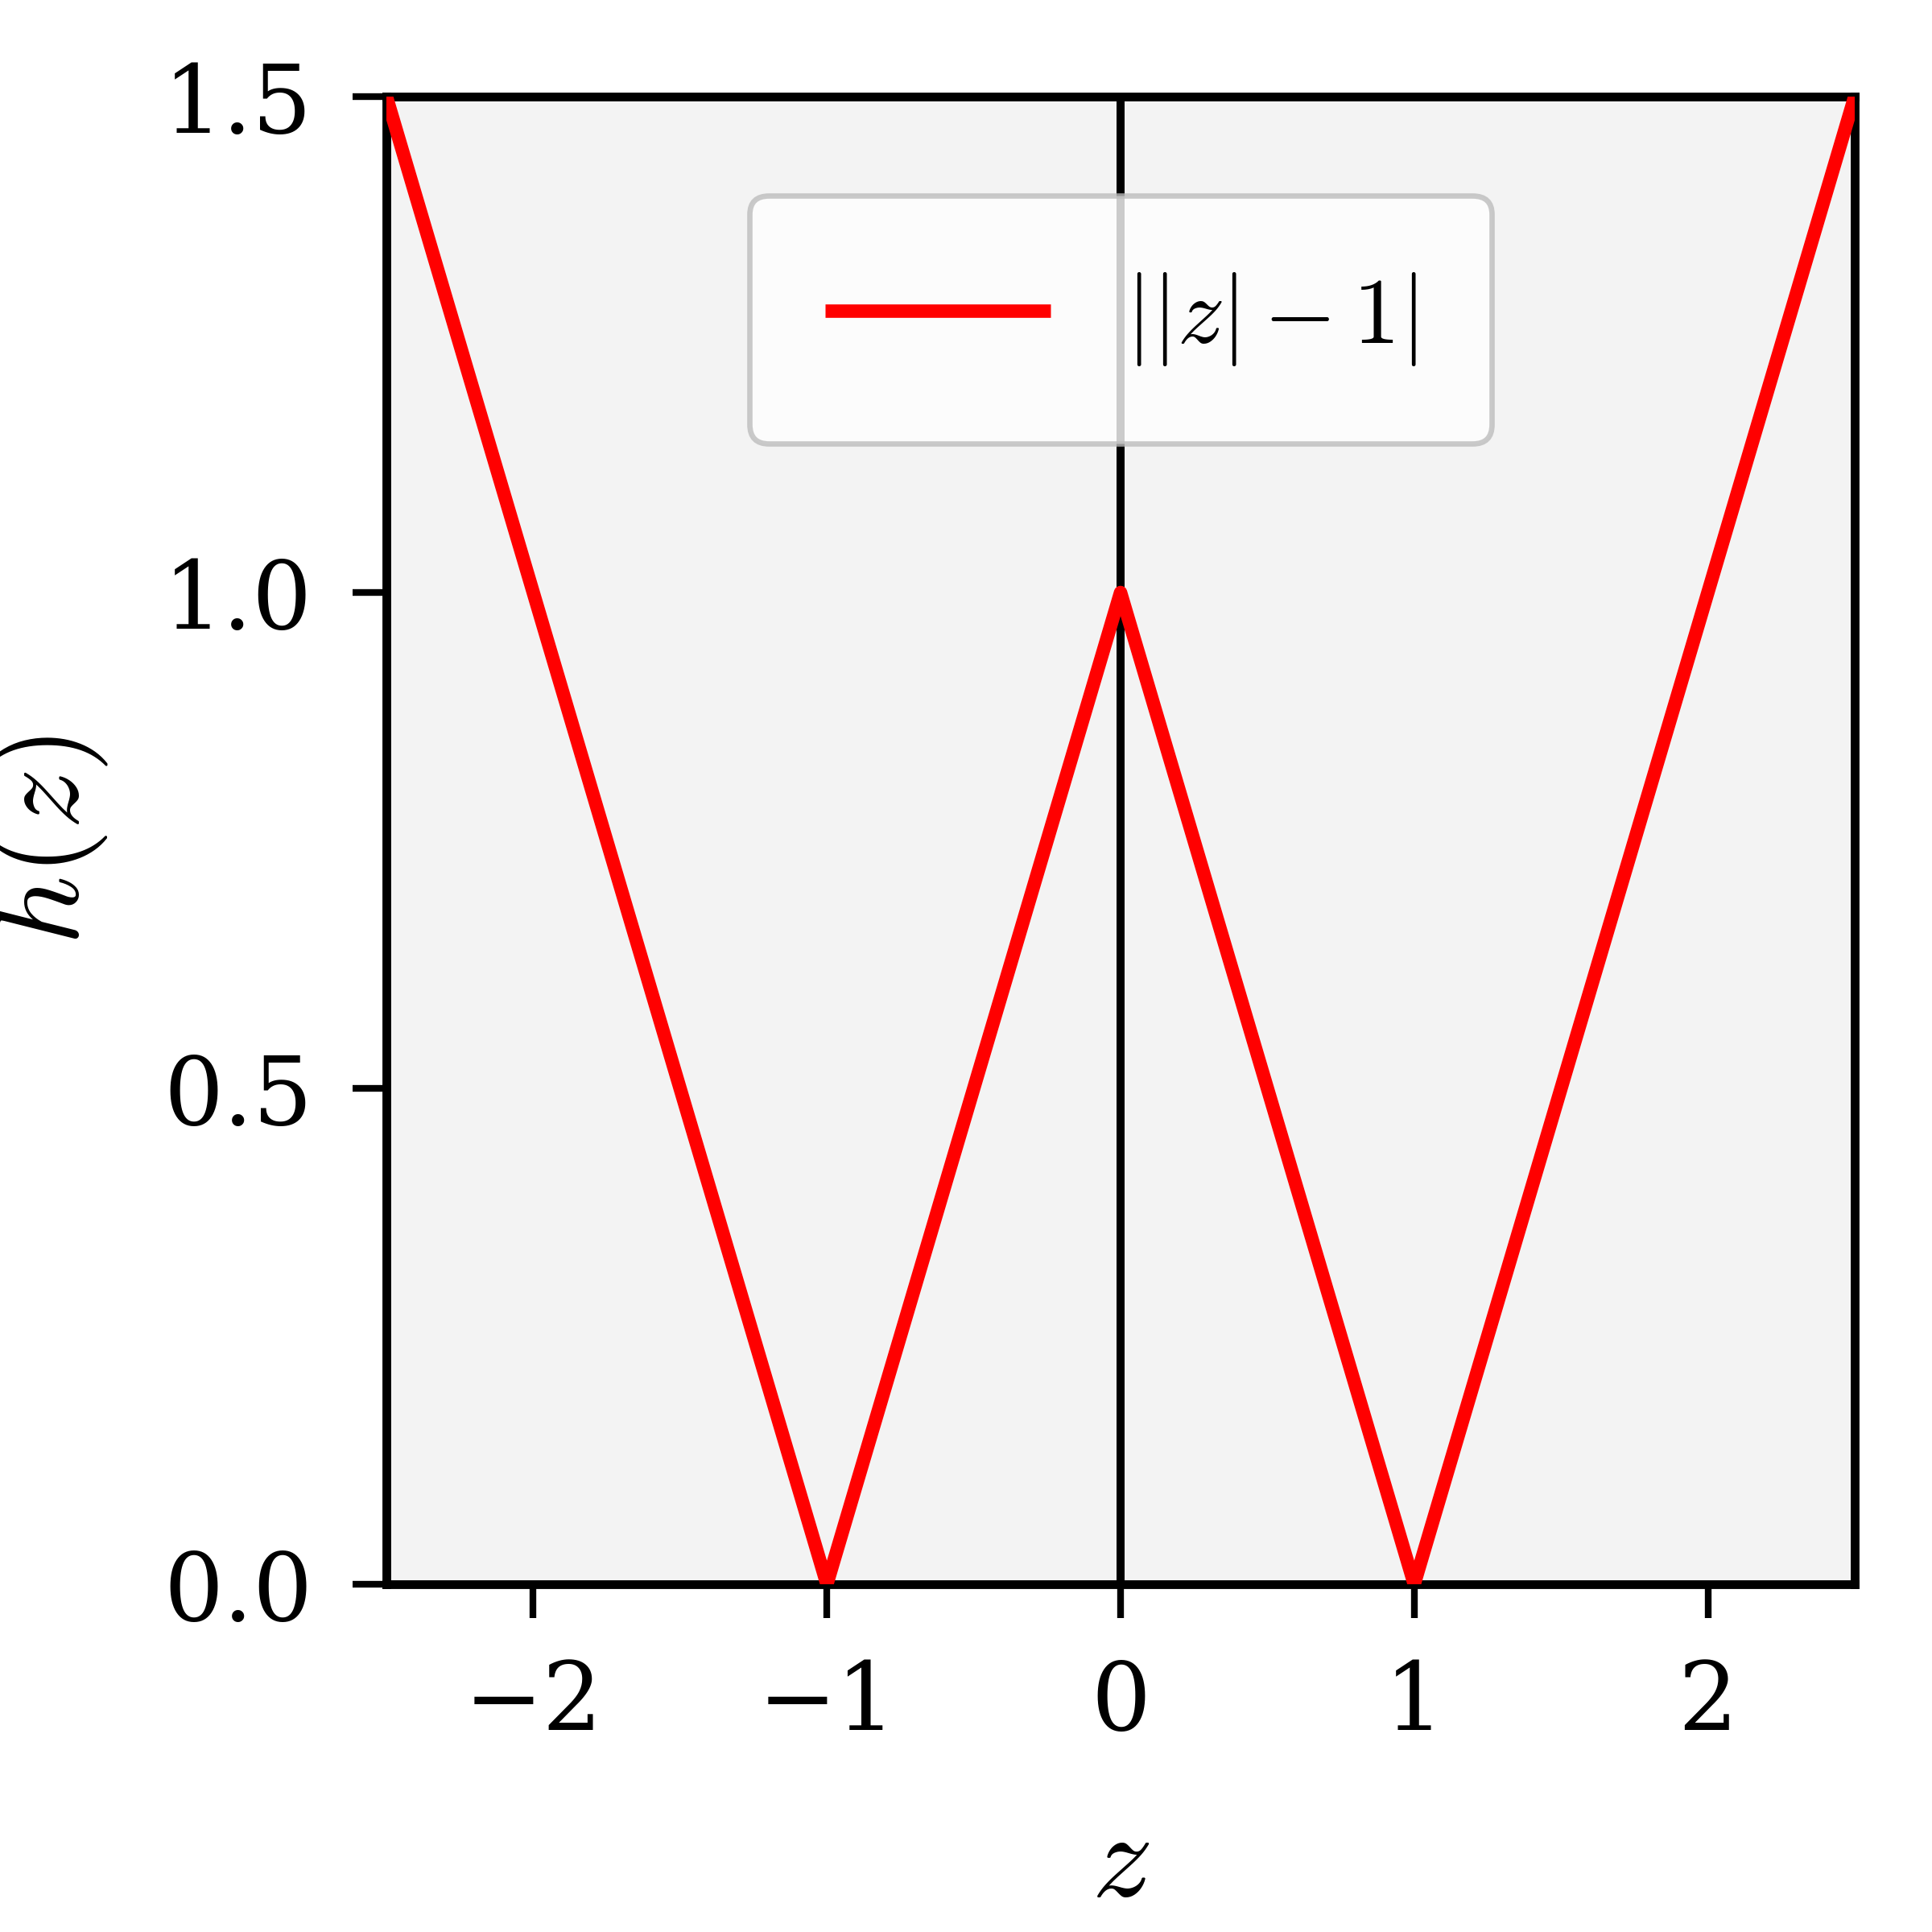
\includegraphics[height=1.85cm,keepaspectratio]{figures/rc1/W_regu.png}\\[-0.12cm]
%   {\scriptsize \(\phi(z)=\lambda\bigl||z|-1\bigr|\)}

%   \column{0.49\linewidth}
%   \centering
%   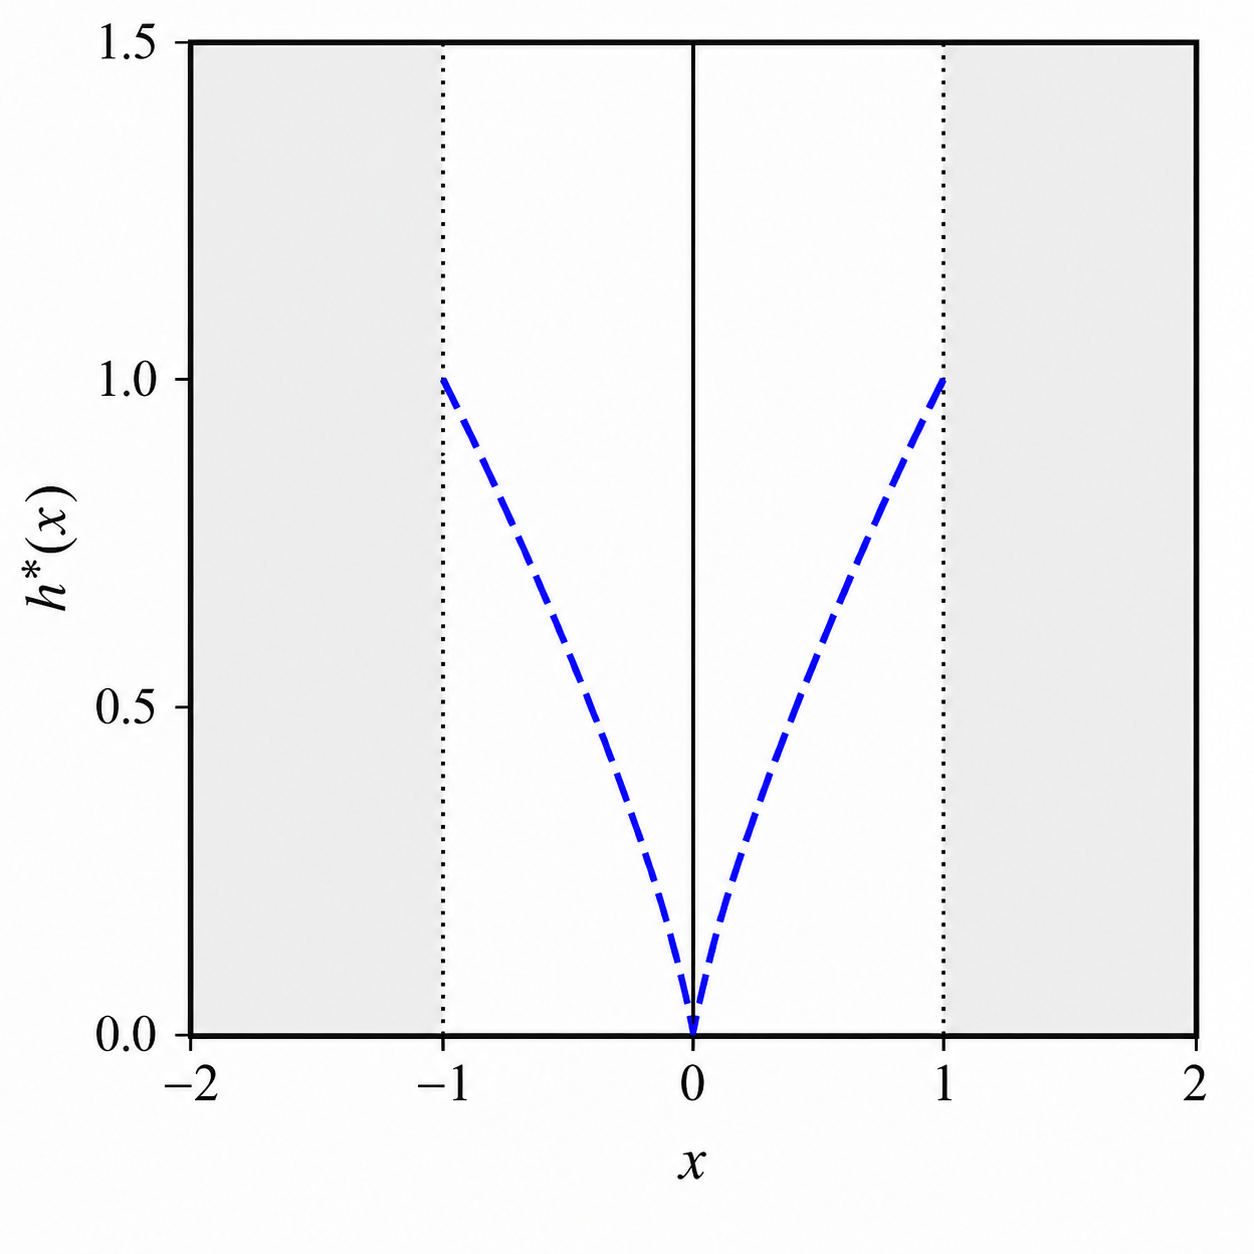
\includegraphics[height=1.85cm,keepaspectratio]{figures/rc1/W-conjugate.png}\\[-0.12cm]
%   {\scriptsize \(\phi^*(y)\)}
% \end{columns}
% \vspace{-0.1cm}
\begin{center}
\begin{tikzpicture}[x=0.62cm,y=0.62cm,>=Stealth,line cap=round,line join=round]
    \begin{scope}[shift={(0,0)}]
        \draw[-{Stealth},thin] (-2.9,0) -- (2.9,0) node[below right] {$b$};
        \draw[-{Stealth},thin] (0,-0.65) -- (0,1.55);
        \draw[line width=0.9pt] (-2.6,1.6) -- (-1,0) -- (0,1) -- (1,0) -- (2.6,1.6);
        \node at (-1,-0.42) {$-1$};
        \node at ( 1,-0.42) {$1$};
        \node at (0,-2) {$\text{(a)}\ h(b)=\lambda_h\bigl||b|-1\bigr|$};
    \end{scope}
    \begin{scope}[shift={(6.5,0)}]
        \draw[-{Stealth},thin] (-2.9,0) -- (2.9,0) node[below right] {$\Lambda$};
        \draw[-{Stealth},thin] (0,-0.65) -- (0,1.55);
        \draw[line width=0.9pt] (-1,1) -- (0,0) -- (1,1);
        \draw[densely dotted,thin] (-1,0) -- (-1,1.5);
        \draw[densely dotted,thin] ( 1,0) -- ( 1,1.5);
        \fill (-1,1) circle (0.07);
        \fill ( 1,1) circle (0.07);
        \node at (-1,-0.42) {$-\lambda_h$};
        \node at ( 1,-0.42) {$\lambda_h$};
        \node at (0,-2) {$\text{(b)}\ h^*(\Lambda)$};
    \end{scope}
    \begin{scope}[shift={(13.0,0)}]
        \draw[-{Stealth},thin] (-2.9,0) -- (2.9,0) node[below right] {$Y$};
        \draw[-{Stealth},thin] (0,-1.35) -- (0,1.35);
        \draw[line width=0.9pt] (-2.8,-1) -- (-2,-1) -- (-1,0) -- (1,0) -- (2,1) -- (2.8,1);
        \draw[densely dotted,thin] (-2,0)--(-2,-1);
        \draw[densely dotted,thin] (-1,0)--(-1,-1);
        \draw[densely dotted,thin] ( 1,0)--( 1, 1);
        \draw[densely dotted,thin] ( 2,0)--( 2, 1);
        \node[below] at (-2,-1.05) {$-(s{+}\lambda_h)$};
        \node at (-1,-0.42) {$-s$};
        \node at ( 1,-0.42) {$s$};
        \node[above] at ( 2,1.05) {$(s{+}\lambda_h)$};
        \node[left] at (0, 1) {$\lambda_h$};
        \node[left] at (0,-1) {$-\lambda_h$};
        \node at (0,-2) {$\text{(c)}\ \prox_{s h^*}(Y)$};
    \end{scope}
\end{tikzpicture}
\end{center}
\vspace{-0.2cm}
\begin{center}
\small Figure 1: A W-type function, its conjugate, and the proximal mapping of $h^*$.
\end{center}

\vspace{0.5cm}

\begin{itemize}
\setlength{\itemsep}{0.04cm}
% $h\circ\bD$ nonseparable in $\bx$
\item \textbf{$h$ nonconvex, }
\(\Longrightarrow\)
\textbf{$h^*$ \blue{convex \& separable}, $\prox_{s h^*}$ \blue{closed-form}}
\vspace{0.24cm}
\[
h^*(\bLmbd)=\sum_{i=1}^n\sum_{j=1}^d h_{ij}^*(\Lambda_{ij}),
\quad
h_{ij}^*(\Lambda_{ij})
=
\begin{cases}
|\Lambda_{ij}|, & |\Lambda_{ij}|\le \lambda_h,\\
+\infty, & |\Lambda_{ij}|>\lambda_h .
\end{cases}
\]

\vspace{-0.1cm}

\[
[\prox_{s h^*}(\bY)]_{ij}
=
\operatorname{sgn}(Y_{ij})\,
\min\big\{(|Y_{ij}|-s)_+,\lambda_h\big\}.
% \qquad s=\tau^{-1}\ \text{in DualHash}.
\]

% \vspace{0.20cm}
% \item \textbf{\(\nabla f_i\), \(\nabla \bc_i\), and
% \(\prox_{\tau \phi^*}\) available}
% \(\Longrightarrow\)
% PDHG [Chambolle and Pock, 2011]

% \[
% \min_{\bx}\; f(\bx)+\phi(\bA\bx)
% \quad\leadsto\quad
% \min_{\bx}\max_{\by}\;
% f(\bx)+\langle \bA\bx,\by\rangle-\blue{\phi^*}(\by).
% \]

% For $h(\bB)=\lambda\bigl||\bB|-\One\bigr|_1=\sum_{i,j}\lambda\bigl||b_{ij}|-1\bigr|$, the conjugate is \blue{element-wise separable}:
% \[
% h^*(\Lambda_{ij})=\begin{cases}|\Lambda_{ij}|, & \Lambda_{ij}\in[-\lambda,\lambda],\\ +\infty, & \text{otherwise}.\end{cases}
% \]


% {\blue{\(\checkmark\)}} {\blue{\textbf{Reformulated quadratic penalty problem:}}} \textbf{Q1 is solved \blue{partially}!}

% \vspace{-0.1cm}

% \[
% (P_\rho)\quad
% \min_{\bx,\bB}\;
% J(\bx,\bB)
% :=
% \underbrace{
% \frac1N\sum_{i=1}^{N} f_i(\bx)
% +\frac{\rho}{2N}\sum_{i=1}^{N}
% \big\|\bc_i(\bx)-\bb_i\big\|^2
% }_{F(\bx,\bB)}
% +
% \underbrace{\sum_{i=1}^{N}\phi(\bb_i)}_{\Phi(\bB)} .
% \]

\end{itemize}

\end{frame}


\begin{frame}{Primal-Dual Hybrid Gradient (PDHG)}
\vspace{0.2cm}

\textbf{PDHG} {\footnotesize [Chambolle and Pock, 2011]} for convex composite optimization:
\[
\min_{\bx}\; f(\bx)+h(\bA\bx)
\quad\overset{h\ \mathrm{convex}}{\Longleftrightarrow}\quad
\min_{\bx}\max_{\by}\; f(\bx)+\langle\bA\bx,\by\rangle-h^*(\by).
\]

\vspace{0.15cm}
\begin{itemize}

% \item[\blue{$\blacktriangleright$}] For convex $h$, $h^*$ is convex and $\prox_{h^*}$ is often \blue{closed-form}.

\vspace{0.2cm}
\item[\blue{$\blacktriangleright$}] \textbf{PDHG} (convex $f$, $h$):
\[
\bx^{k+1}=\prox_{\sigma f}\!\bigl(\bx^k-\sigma\bA^\top\by^k\bigr),
\]
\[
\by^{k+1}=\prox_{\tau h^*}\!\bigl(\by^k+\tau\bA(\bx^{k+1}+\theta(\bx^{k+1}-\bx^k))\bigr), 0 < \theta \leq 1.
\]
With $\theta=1$ and $\sigma\tau\|\bA\|^2<1$, the ergodic primal-dual gap is $O(1/k)$.

% \item[\blue{$\blacktriangleright$}] \textbf{PPDG} {\footnotesize [Guo, 2026]}
% (fully nonconvex):
\[
\bx^{k+1}=\bx^k-\sigma\bigl(\nabla f(\bx^k)+\bA^\top\by^k\bigr),\quad
\by^{k+1}=\prox_{h^*}^{\bM}\!\bigl(\by^k+\bM^{-1}\bA(2\bx^{k+1}-\bx^k)\bigr),
\]
converges to a critical point with $\bM=\sigma\bA\bA^\top$.
% \item[\blue{$\blacktriangleright$}] \red{Gap:} No \red{non-asymptotic stochastic oracle complexity}
% for an $\epsilon$-stationary point in the fully nonconvex setting.
\end{itemize}
\end{frame}


\section{DualHash: A Stochastic Primal-Dual Algorithm}

\begin{frame}{DualHash: Three-Block Update Framework}
\vspace{0.15cm}

\begin{align}
\max_{\bLmbd}\min_{\bx,\,\bB,\,\bY}\;&F(\bx,\bB)+h(\bY)+\langle\bLmbd,\bB-\bY\rangle \notag\\
% &= \max_{\bLmbd}\min_{\bx,\,\bB}\;F(\bx,\bB)+\langle\bLmbd,\bB\rangle + \min_{\bY}\{h(\bY)-\langle\bLmbd,\bY\rangle\} \notag\\
&= \max_{\bLmbd}\min_{\bx,\,\bB}\;F(\bx,\bB)+\langle\bLmbd,\bB\rangle - h^*(\bLmbd), \tag{D}
% \label{eq:dual}
\end{align}

\nii\textbf{Idea:} Employ an alternating update scheme for $(\bx,\bB,\bLmbd)$.

\vspace{0.15cm}
\begin{itemize}
\item[\blue{$\triangleright$}] \textbf{$\bx$-update (stochastic gradient descent on $\calL$):}
\[
\bx^{k+1} = \bx^k - \eta_k\,\widetilde\nabla_{\bx} F(\bx^k,\bB^k),
\]
where $\widetilde\nabla_{\bx} F$ uses \blue{inertial acceleration} or \blue{variance reduction}.

% condition number = 1;
\vspace{0.15cm}
\item[\blue{$\triangleright$}] 
%min \| \bB - (\bB^k - 1/tau \nabla_B F)\|^2
% \textbf{$\bB$-update (gradient descent on $\calL$):}
\[
\bB^{k+1} = \bB^k - \tau\bigl(\nabla_{\bB} F(\bx^{k+1},\bB^k) + \bLmbd^k\bigr).
\]

\vspace{0.15cm}
\item[\blue{$\triangleright$}] \textbf{$\bLmbd$-update (proximal ascent with extrapolation):}
\[
\bLmbd^{k+1} = \prox_{\tau^{-1} h^*}\!\bigl(\bLmbd^k + \tau^{-1}(2\bB^{k+1}-\bB^k)\bigr).
\]
\end{itemize}

\vspace{0.1cm}
\begin{block}{Key ingredients}
The $\bx$-update admits two variants: \textbf{DualHash-StoM} (inertial) and \textbf{DualHash-StoRM} (recursive momentum).
\end{block}
\end{frame}


\begin{frame}{DualHash-StoM}
\vspace{0.1cm}
% \small

\nii\textbf{Momentum estimator} at the extrapolated point $\bz^k=\bx^k+\beta_k(\bx^k-\bx^{k-1})$:
\[
\bG^k = \nabla_{\bx} F(\bz^k,\bB^k;\calJ_k),
\qquad
\bx^{k+1} = \by^k - \eta_k \bG^k,
\quad \by^k=\bx^k+\alpha_k(\bx^k-\bx^{k-1}).
\]

\vspace{-0.1cm}
\begin{algorithmic}[1]
\REQUIRE $\bx^1=\bz^1=\by^1\in\RR^{d_{\bx}}$, $\bB^1,\bLmbd^1\in\RR^{n\times d}$; parameters $\{\eta_k\}$, $\tau$, $b_k$, $\{\alpha_k,\beta_k\in(0,1)\}$.
\FOR{$k=1,2,\ldots$}
  \STATE Sample mini-batch $\calJ_k\subseteq\{1,\dots,n\}$, $|\calJ_k|=b_k$.
  \STATE $\bG^k=\nabla_{\bx} F(\bz^k,\bB^k;\calJ_k)$, \;\; $\bx^{k+1}=\by^k-\eta_k\bG^k$.
  \STATE $\bB^{k+1}=\bB^k-\tau(\nabla_{\bB}F(\bx^{k+1},\bB^k)+\bLmbd^k)$.
  \STATE $\bLmbd^{k+1}=\prox_{\tau^{-1}h^*}(\bLmbd^k+\tau^{-1}(2\bB^{k+1}-\bB^k))$.
\ENDFOR
\ENSURE $(\bx^R,\bB^R,\bLmbd^R)$, $R\sim\mathrm{Unif}\{2,\dots,T+1\}$.
\end{algorithmic}

% \vspace{0.1cm}
% \begin{remark}
% Nesterov acceleration: $\alpha_k=\beta_k\neq 0$; heavy-ball: $\beta_k=0$; vanilla SGD: $\alpha_k=\beta_k=0$.
% \end{remark}
\end{frame}


\begin{frame}{DualHash-StoRM}
\vspace{0.1cm}
% \small

\nii\textbf{Recursive momentum (StoRM) estimator:}\footnote{A. Cutkosky and F. Orabona. Momentum-based variance reduction in non-convex SGD. NeurIPS, 2019: 15236--15245.}
\[
\bD^k =
\begin{cases}
\nabla_{\bx} F(\bx^1,\bB^1;\calJ_1), & k=1,\\
\nabla_{\bx} F(\bx^k,\bB^k;\calJ_k) + (1-\rho_{k-1})\bigl(\bD^{k-1}-\nabla_{\bx} F(\bx^{k-1},\bB^{k-1};\calJ_k)\bigr), & k>1.
\end{cases}
\]

\vspace{-0.1cm}
\begin{algorithmic}[1]
\REQUIRE $\bx^1\in\RR^{d_{\bx}}$, $\bB^1,\bLmbd^1\in\RR^{n\times d}$; parameters $\{\eta_k\}$, $\tau$, $b_k$, $\{\rho_k\in(0,1)\}$.
\FOR{$k=1,2,\ldots$}
  \STATE Sample mini-batch $\calJ_k$; compute $\bD^k$.
  \STATE $\bx^{k+1}=\bx^k-\eta_k\bD^k$.
  % \STATE $\bB^{k+1}=\bB^k-\tau(\nabla_{\bB}F(\bx^{k+1},\bB^k)+\bLmbd^k)$.
  % \STATE $\bLmbd^{k+1}=\prox_{\tau^{-1}h^*}(\bLmbd^k+\tau^{-1}(2\bB^{k+1}-\bB^k))$.
\ENDFOR
\ENSURE $(\bx^R,\bB^R,\bLmbd^R)$, $R\sim\mathrm{Unif}\{2,\dots,T+1\}$.
\end{algorithmic}

\begin{block}{Remark}
Variance reduction \blue{without} full-gradient or large-batch computation.
\end{block}
\end{frame}

\section{Complexity Results}

\begin{frame}[t]{Main Assumptions}
% \small
\vspace{0.2cm}
\begin{equation}
  \quad
\max_{\bLmbd}\min_{\bx,\bB}\;
\calL(\bx,\bB,\bLmbd)
:=
F(\bx,\bB)
+\langle\bB,\bLmbd\rangle
-h^*(\bLmbd), \tag{D}
\end{equation}


\vspace{0.2cm}
\nii\textbf{AS.1}
\begin{itemize}
\item[(i)] The objective of Problem (P) is lower bounded by $J^*$.
\item[(ii)] $F(\bx,\bB)$ is $L_F=\calO(1)$-smooth w.r.t.\ $(\bx,\bB)$.
\item[(iii)] For $i\sim\mathrm{Uniform}\{1,\dots,n\}$: $\EE_i[\nabla_{\bx}F_i(\bx,\bb_i)]=\nabla_{\bx}F(\bx,\bB)$ and $\EE_i[\|\nabla_{\bx}F_i-\nabla_{\bx}F\|^2]\le\sigma^2$.
\end{itemize}

\vspace{0.2cm}
\textbf{AS.2 (Mean-squared smoothness).}
\[
\EE_i\!\left[\|\nabla_{\bx}F_i(\bx,\bb_i)-\nabla_{\bx}F_i(\bx',\bb_i')\|^2\right]\le L_F^2\!\left[\|\bx-\bx'\|^2+\|\bB-\bB'\|^2\right],
\]
Here, $\bb_i$ and $\bb_i'$ denote the $i$-th rows of $\bB$ and $\bB'$, respectively.

\vspace{0.2cm}
\begin{remark}
$L_F$ remains $\calO(1)$, as the penalty formulation cancels the potential $\calO(\sqrt{n})$ scaling.
\end{remark}
\end{frame}

\begin{frame}[t]{Convergence Criterion: Stochastic $\varepsilon$-Critical Point}
% \small
\vspace{0.2cm}

\begin{itemize}
  \item A primal--dual triple $(\bar{\bx},\bar{\bB},\bar{\bLmbd})$ is a
  critical point of Problem $(P)$ if
  $\bm{0}\in\partial\calL(\bar{\bx},\bar{\bB},\bar{\bLmbd})$.
  \item A random output $(\bx^R,\bB^R,\bLmbd^R)$ is called a stochastic
  $\varepsilon$-critical point of Problem $(P)$ if
% \vspace{-0.10cm}

\begin{equation}\label{equ:esp}
\EE\!\left[
\operatorname{dist}^2
\bigl(\bm{0},\partial\calL(\bx^R,\bB^R,\bLmbd^R)\bigr)
\right]
\le \varepsilon^2,
\end{equation}
% i.e.,
% \vspace{-0.24cm}
% \[
% \begin{aligned}
% \left[
% \EE\!\left[
% \|\nabla_{\bx}F(\bx^R,\bB^R)\|^2
% +
% \|\nabla_{\bB}F(\bx^R,\bB^R)+\bLmbd^R\|^2
% \right]
% \right]^{1/2}
% &\le \varepsilon,\\
% \left[
% \EE\!\left[
% \operatorname{dist}^2
% \!\left(\bB^R,\partial h^*(\bLmbd^R)\right)
% \right]
% \right]^{1/2}
% &\le \varepsilon .
% \end{aligned}
% \]

\item Our goal is to establish the stochastic first oracle (SFO) complexity of finding 
stochastic $\varepsilon$-critical points.

\end{itemize}


\vspace{0.04cm}
\begin{block}{Lemma 5.2 [LWC26]\textsuperscript{1}}
Under Assumption (i), if
$(\bx^*,\bB^*,\bLmbd^*)$ is an optimal solution of Problem $(P)$
and its dual $(D)$, then
$\bm{0}\in \partial\calL(\bx^*,\bB^*,\bLmbd^*).$
\end{block}
\end{frame}

% \begin{frame}[t]{Proof Sketch of Lemma 5.2}
% \vspace{0.20cm}

% {\blue{\textbf{1. Saddle-point characterization.}}}
% By Theorem 2.158\footnote{\scriptsize Bonnans J. F., Shapiro A. Perturbation analysis of optimization problems. Springer, 2013.}, primal--dual optimality yields
% \[
% (\bx^*,\bB^*)\in\argmin_{\bx,\bB}\calL(\bx,\bB,\bLmbd^*),
% \qquad
% h(\bB^*)+h^*(\bLmbd^*)
% =\langle\bLmbd^*,\bB^*\rangle.
% \]

% \vspace{0.12cm}
% {\blue{\textbf{2. Block optimality conditions.}}}
% The first relation and the smoothness of $F$ give
% \[
% \nabla_{\bx}F(\bx^*,\bB^*)=0,
% \qquad
% \nabla_{\bB}F(\bx^*,\bB^*)+\bLmbd^*=0.
% \]
% The Fenchel--Young equality further implies
% \[
% \bB^*\in\partial h^*(\bLmbd^*).
% \]

% \vspace{0.12cm}
% {\blue{\textbf{3. Criticality.}}}
% Combining the three block conditions gives
% \[
% {\blue{\bm{0}\in\partial\calL(\bx^*,\bB^*,\bLmbd^*)}}.
% \]
% \end{frame}

% \begin{frame}{Complexity Analysis Framework}
% \vspace{0.2cm}

% \begin{columns}[T,onlytextwidth]
% \begin{column}{0.46\textwidth}
% \vspace{0.2cm}
% The analysis proceeds in four stages:

% \vspace{0.2cm}
% \begin{enumerate}
% \item \textbf{Bounded iterates:} $\{(\bx^k,\bB^k,\bLmbd^k)\}$ is bounded (coercivity + $\bLmbd^k\in[-\lambda,\lambda]$).
% \item \textbf{Dual boundedness:} $\|\bLmbd^{k+1}-\bLmbd^k\|^2$ controlled by primal residuals.
% \item \textbf{Lyapunov descent:} construct $\Psi_m$ or $\Psi_r$ to obtain approximate sufficient descent.
% \item \textbf{Oracle complexity:} balance parameters to reach $\varepsilon$-criticality.
% \end{enumerate}
% \end{column}

% \begin{column}{0.52\textwidth}
% \centering
% 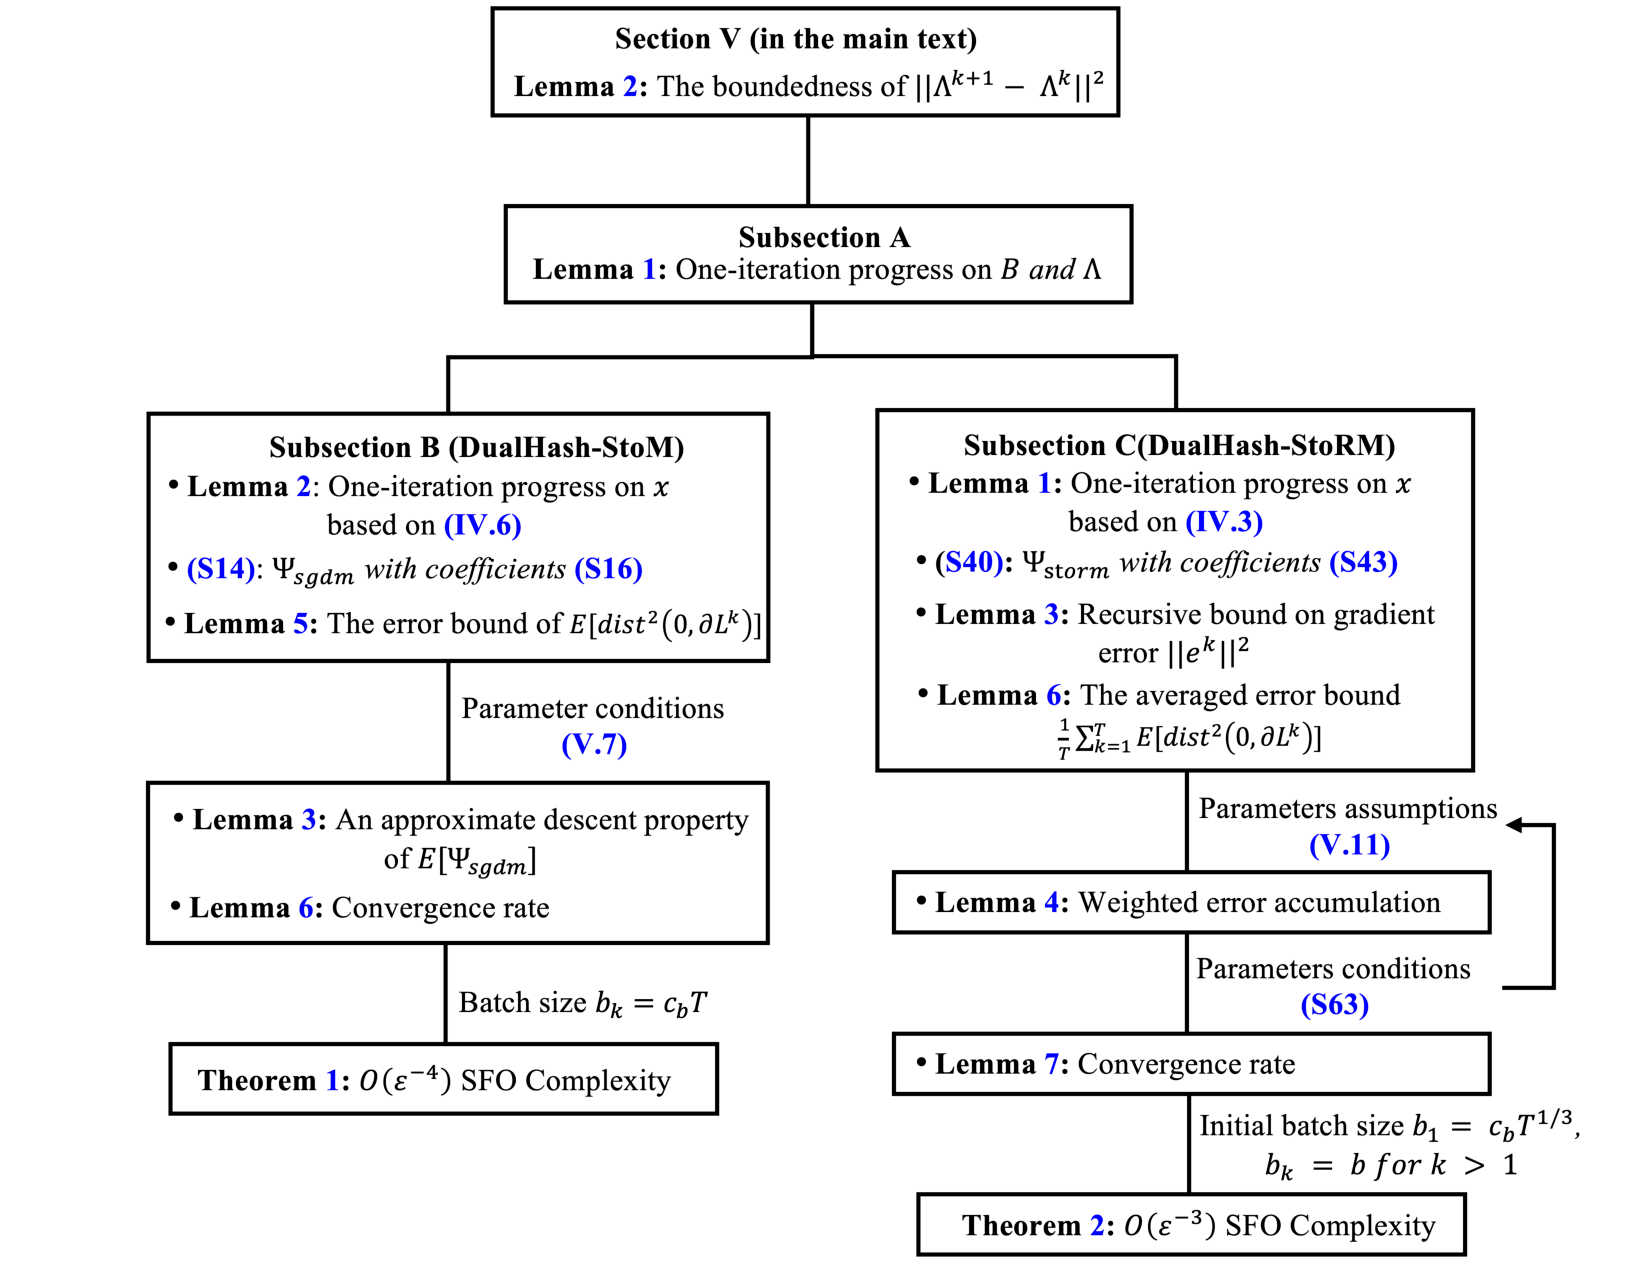
\includegraphics[width=\textwidth,height=0.72\textheight,keepaspectratio]{papers_img/proof_framework.pdf}
% \end{column}
% \end{columns}
% \end{frame}


\begin{frame}{Oracle Complexity of DualHash-StoM}
\vspace{0.2cm}
\small

\nii\textbf{Lyapunov function:}
\[
\Psi_m(\calQ^k)=\calL(\bx^k,\bB^k,\bLmbd^k)-C_1\Delta_{\bB}^{k+1}+C_2\Delta_{\bB}^k-C_3\Delta_{\bx}^{k+1}+C_4\Delta_{\bx}^k.
\]
\[
\calQ^k:=\bigl\{\bx^k,\bB^k,\bLmbd^k,\bB^{k+1},\bB^{k-1},\bx^{k+1},\bx^{k-1}\bigr\},
\qquad \{\calQ^k\}_{k\in\mathbb{N}}.
\]

\nii\textbf{Parameter setting:}
\begin{equation}
  \eta_k=\frac{\eta}{L_F},\quad \alpha_k=\alpha,\quad \beta_k=\beta,\quad \tau\le\frac{\sqrt{\tilde\delta}}{L_F},\quad b_k=b=c_b T. \tag{S.1}
\end{equation}
\vspace{0.2cm}
\begin{block}{Theorem 1 (DualHash-StoM)}
Under AS.1 and condition (S.1), there exists $R\sim\mathrm{Unif}\{2,\dots,T+1\}$ such that $(\bx^R,\bB^R,\bLmbd^R)$ satisfies \eqref{equ:esp} with
\[
T=\left\lceil\frac{L_\Delta\Delta_1+C_\sigma\sigma^2/c_b}{\varepsilon^2}\right\rceil.
\]
The total number of SFO calls is \blue{$\calO(\varepsilon^{-4})$}.
\end{block}
\end{frame}


\begin{frame}{Oracle Complexity of DualHash-StoRM}
\vspace{0.2cm}
\small

\nii\textbf{Lyapunov function:}
\[
\Psi_r(\calQ^k)=\calL(\bx^k,\bB^k,\bLmbd^k)-C_1\Delta_{\bB}^{k+1}+C_2\Delta_{\bB}^k-C_3\Delta_{\bx}^{k+1}.
\]

\nii\textbf{Parameter setting:}
\begin{equation}
  \eta_k=\frac{\eta}{\tilde L_F T^{1/3}},\quad \rho_k=\frac{8\rho\eta^2}{T^{2/3}},\quad \tau\le\frac{\sqrt{\tilde\delta}}{L_F},\quad b_1=c_b T^{1/3}, \quad b_k = \calO(1).  \tag{S.2}
\end{equation}

\vspace{0.2cm}
\begin{block}{Theorem 2 (DualHash-StoRM)}
Under AS.1(i), (iii), AS.2 and condition (S.2), there exists $R\sim\mathrm{Unif}\{2,\dots,T+1\}$ such that $(\bx^R,\bB^R,\bLmbd^R)$ satisfies \eqref{equ:esp} with
\[
T=\left\lceil\frac{\bigl(\tilde L_\Delta\tilde\Delta_1+\tilde C_\sigma(\frac{\sigma^2}{4\rho\eta^2 c_b}+\frac{32\rho\eta^2\sigma^2}{b})\bigr)^{3/2}}{\varepsilon^3}\right\rceil.
\]
The total number of SFO calls is \blue{$\calO(\varepsilon^{-3})$}.
\end{block}
\end{frame}


\begin{frame}{Complexity Results}
\vspace{0.3cm}

\begin{center}
\begin{tabular}{lccl}
\toprule
\textbf{Algorithm} & \textbf{Assumptions} & \textbf{Complexity} & \textbf{Remark} \\
\midrule
SPGD (one-block)\footnotemark[1] & AS.1 & $\calO(\varepsilon^{-4})$ & standard baseline \\
VR-SPGD (one-block)\footnotemark[2] & AS.1, AS.2 & $\Omega (\varepsilon^{-3})$ & lower bound \\
\midrule
DualHash-StoM & AS.1 & \blue{$\calO(\varepsilon^{-4})$} & multi-block primal-dual \\
DualHash-StoRM & AS.1, AS.2 & \blue{$\calO(\varepsilon^{-3})$} & matches lower bound \\
\bottomrule
\end{tabular}
\end{center}

\footnotetext[1]{Ghadimi S., Lan G., Zhang H. Mini-batch stochastic approximation methods for nonconvex stochastic composite optimization. Mathematical Programming, 2016, 155(1--2): 267--305.}
\footnotetext[2]{Arjevani Y. et al. Lower bounds for non-convex stochastic optimization. Mathematical Programming, 2023, 199(1): 165--214.}

\vspace{0.4cm}
\begin{center}
\blue{\textbf{Key point.}} Despite tackling a multi-block primal-dual problem, DualHash \blue{preserves the nearly optimal $\varepsilon$-dependence} without degradation.
\end{center}
\end{frame}


\section{Numerical Experiments}

\begin{frame}{Experimental Setup}
% \small

We evaluate on \textbf{CIFAR-10}, \textbf{NUS-WIDE}, and \textbf{ImageNet-100}, covering single-label, multi-label, and large-scale image retrieval settings.

\begin{itemize}
\item[\blue{$\blacktriangleright$}] \textbf{Problem.} For \(s^h_{ij}=\tfrac12\langle\bu_i,\bu_j\rangle\) and \(\bu_i=\tanh(\bC(\bx;\ba_i))\), the pairwise objective is
\begin{align*}
\min_{\bx,\bB}\quad
&-\frac{1}{|\mathcal{S}|}\sum_{s^o_{ij}\in\mathcal{S}}
\log\!\left(1+\exp\!\left(-\alpha s^o_{ij}s^h_{ij}\right)\right)\\[-1mm]
&+\frac{\gamma}{2n}\sum_{i=1}^n\|\bb_i-\bu_i\|_2^2
 +\sum_{i=1}^n\lambda\|\,|\bb_i|-\bm{1}\,\|_1.
\end{align*}
\item[\blue{$\blacktriangleright$}] \textbf{Baselines.} We compare with three groups of methods:
(i) \textbf{SDH} as the discrete hashing baseline;
(ii) \textbf{W-type regularization methods}: DHN~\blue{[ZLWC16]}, DSH~\blue{[LWSC16]}, DTSH~\blue{[WSK16]}, and MDSHC~\blue{[WPLLYL23]};
(iii) \textbf{quantization-error-oriented methods}: HashNet~\blue{[CLWY17]}, DSDH~\blue{[LSHT17]}, and OrthoHash~\blue{[HNZCSX21]}.
\item[\blue{$\blacktriangleright$}] \textbf{Backbones.} AlexNet and ResNet-50, with ELU activation.
\item \textbf{Metrics.} mAP, P@topK, P@r=2, and quantization error.
\end{itemize}
\end{frame}


% Original convergence-validation slide retained for reference.
% \begin{frame}{Convergence Validation}
% \vspace{0.1cm}
% \begin{center}
% 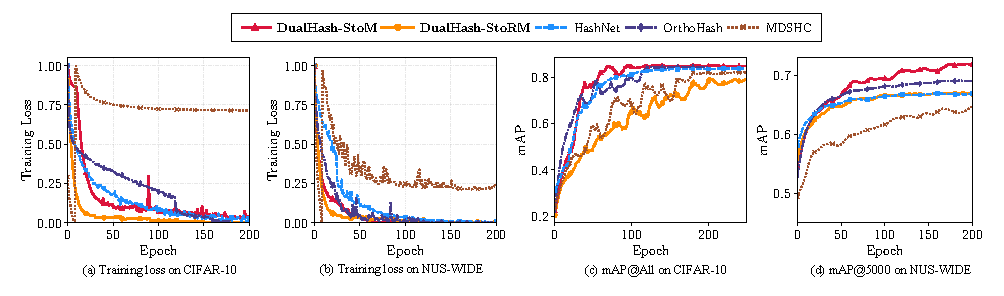
\includegraphics[width=0.92\textwidth,height=0.72\textheight,keepaspectratio]{results_images/ex1_4figures_new.pdf}
% \end{center}
% \vspace{-0.1cm}
% \begin{center}
% \footnotesize Figure 2: Training loss and mAP curves of DualHash and baselines (64-bit) on CIFAR-10 and NUS-WIDE.
% \end{center}
% \end{frame}


\begin{frame}{mAP Results: AlexNet}
\vspace{0.15cm}
% map \right 1, better
\begin{center}
\renewcommand{\arraystretch}{1.25}
\resizebox{0.96\textwidth}{!}{%
\begin{tabular}{lcccccc}
\toprule
\multirow{2}{*}{\textbf{Method}} & \multicolumn{3}{c}{\textbf{CIFAR-10}} & \multicolumn{3}{c}{\textbf{NUS-WIDE}} \\
\cmidrule(lr){2-4} \cmidrule(lr){5-7}
& 32 bits & 48 bits & 64 bits & 32 bits & 48 bits & 64 bits \\
\midrule
DSH~\blue{[LWSC16]} & 0.7530 & 0.7817 & 0.8010 & 0.6629 & 0.6617 & 0.6634 \\
OrthoHash~\blue{[HNZCSX21]} & 0.8059 & 0.8387 & 0.8355 & 0.6912 & 0.7083 & 0.7176 \\
MDSHC~\blue{[WPLLYL23]} & 0.8238 & 0.8350 & 0.8262 & 0.6452 & 0.6081 & 0.6493 \\
\cmidrule(lr){1-7}
\textbf{DualHash-StoM} & \textbf{0.8481} & \textbf{0.8534} & \textbf{0.8539} & \textbf{0.7002} & \textbf{0.7248} & \textbf{0.7448} \\
\bottomrule
\end{tabular}}
\end{center}
\vspace{0.25cm}
\begin{itemize}
\item DualHash-StoM achieves the \blue{best mAP} across all selected code lengths on both datasets.
\end{itemize}
\end{frame}


\begin{frame}{mAP Results: ResNet-50}
\vspace{0.15cm}
\begin{center}
\renewcommand{\arraystretch}{1.25}
\resizebox{0.96\textwidth}{!}{%
\begin{tabular}{lcccccc}
\toprule
\multirow{2}{*}{\textbf{Method}} & \multicolumn{3}{c}{\textbf{CIFAR-10}} & \multicolumn{3}{c}{\textbf{NUS-WIDE}} \\
\cmidrule(lr){2-4} \cmidrule(lr){5-7}
& 32 bits & 48 bits & 64 bits & 32 bits & 48 bits & 64 bits \\
\midrule
DSH~\blue{[LWSC16]} & 0.8116 & 0.8217 & 0.8239 & 0.6952 & 0.6981 & 0.7165 \\
OrthoHash~\blue{[HNZCSX21]} & 0.9182 & 0.9202 & 0.9224 & 0.7600 & 0.7569 & 0.7863 \\
MDSHC~\blue{[WPLLYL23]} & 0.9007 & 0.9063 & 0.9227 & 0.7002 & 0.7248 & 0.7758 \\
\cmidrule(lr){1-7}
\textbf{DualHash-StoM} & \textbf{0.9202} & \textbf{0.9392} & \textbf{0.9416} & \textbf{0.7783} & \textbf{0.7721} & \textbf{0.8016} \\
\bottomrule
\end{tabular}}
\end{center}
\vspace{0.25cm}
\begin{itemize}
\item ResNet-50 strengthens the retrieval performance gap, with DualHash-StoM remaining better.
% (number)
\end{itemize}
\end{frame}


% \begin{frame}{mAP Results: ImageNet-100}
% \vspace{0.15cm}
% \begin{center}
% \renewcommand{\arraystretch}{1.35}
% \resizebox{0.72\textwidth}{!}{%
% \begin{tabular}{lcc}
% \toprule
% \multirow{2}{*}{\textbf{Method}} & \multicolumn{2}{c}{\textbf{ImageNet-100 (ResNet-50)}} \\
% \cmidrule(lr){2-3}
% & 48 bits & 64 bits \\
% \midrule
% DSH~\blue{[LWSC16]} & 0.7335 & 0.7585 \\
% OrthoHash~\blue{[HNZCSX21]} & 0.8510 & 0.8636 \\
% MDSHC~\blue{[WPLLYL23]} & 0.8561 & 0.8657 \\
% \cmidrule(lr){1-3}
% \textbf{DualHash-StoM} & \textbf{0.8662} & \textbf{0.8714} \\
% \bottomrule
% \end{tabular}}
% \end{center}
% \vspace{0.35cm}
% \begin{itemize}
% \item DualHash-StoM achieves the \blue{best mAP} at both 48 and 64 bits on ImageNet-100.
% \item The gain over the strongest baseline MDSHC is \blue{1.01} and \blue{0.57} percentage points, respectively.
% \end{itemize}
% \end{frame}


% \begin{frame}{Retrieval Performance: CIFAR-10}
% \vspace{0.05cm}
% \begin{center}
% % Shared legend extracted from Figure 6.2.
% 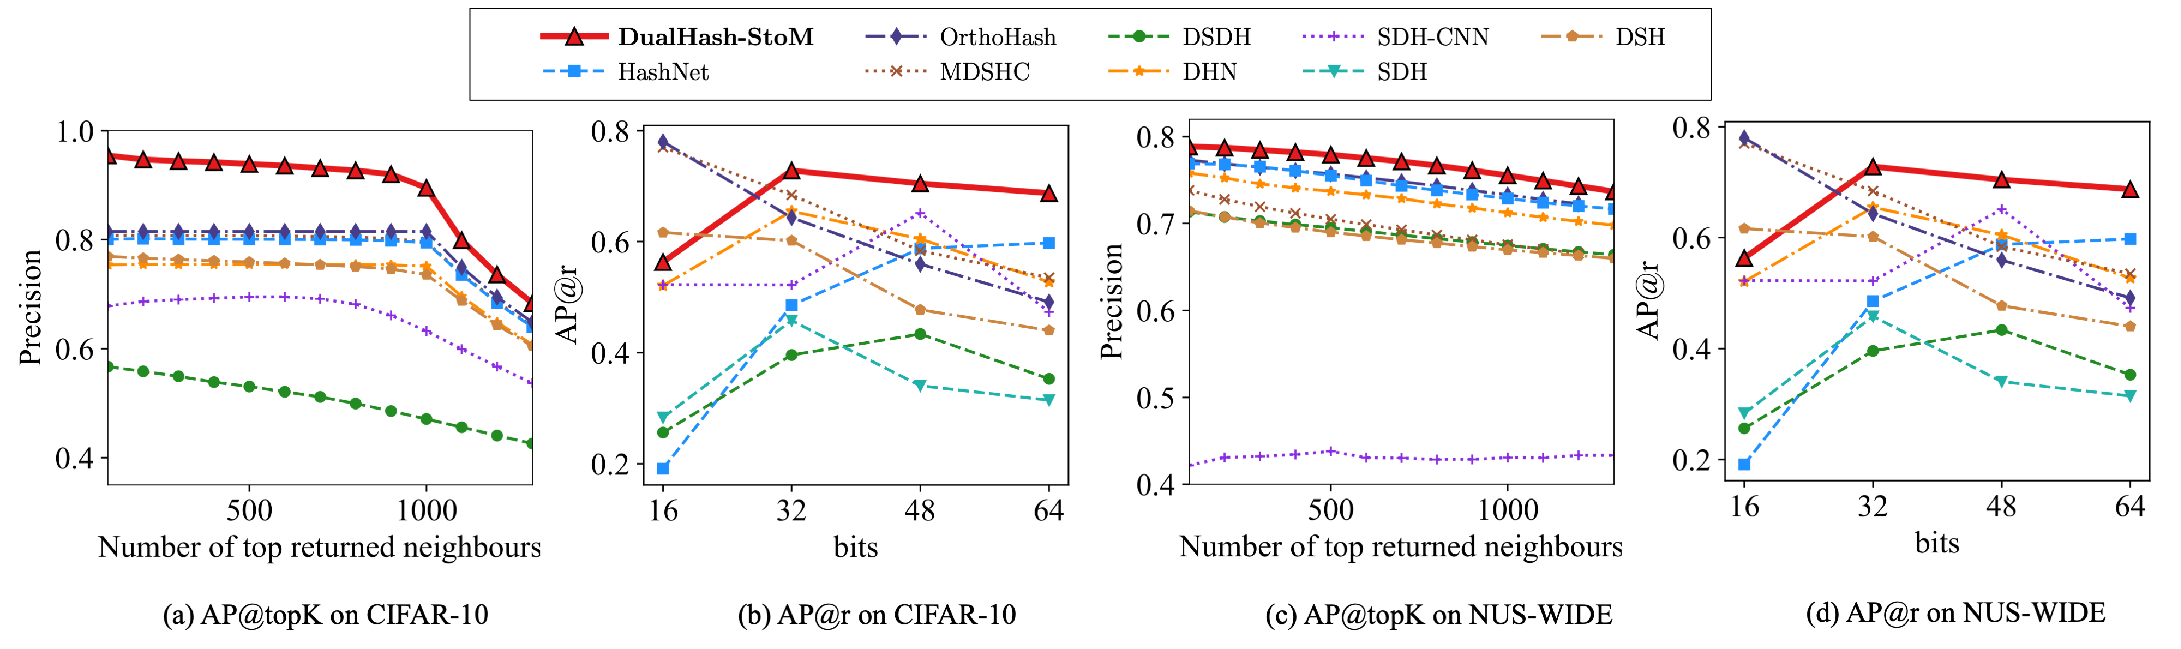
\includegraphics[width=0.76\textwidth,trim=200 264 200 0,clip]{results_images/ex2_4figures.pdf}
% \\[-0.02cm]
% 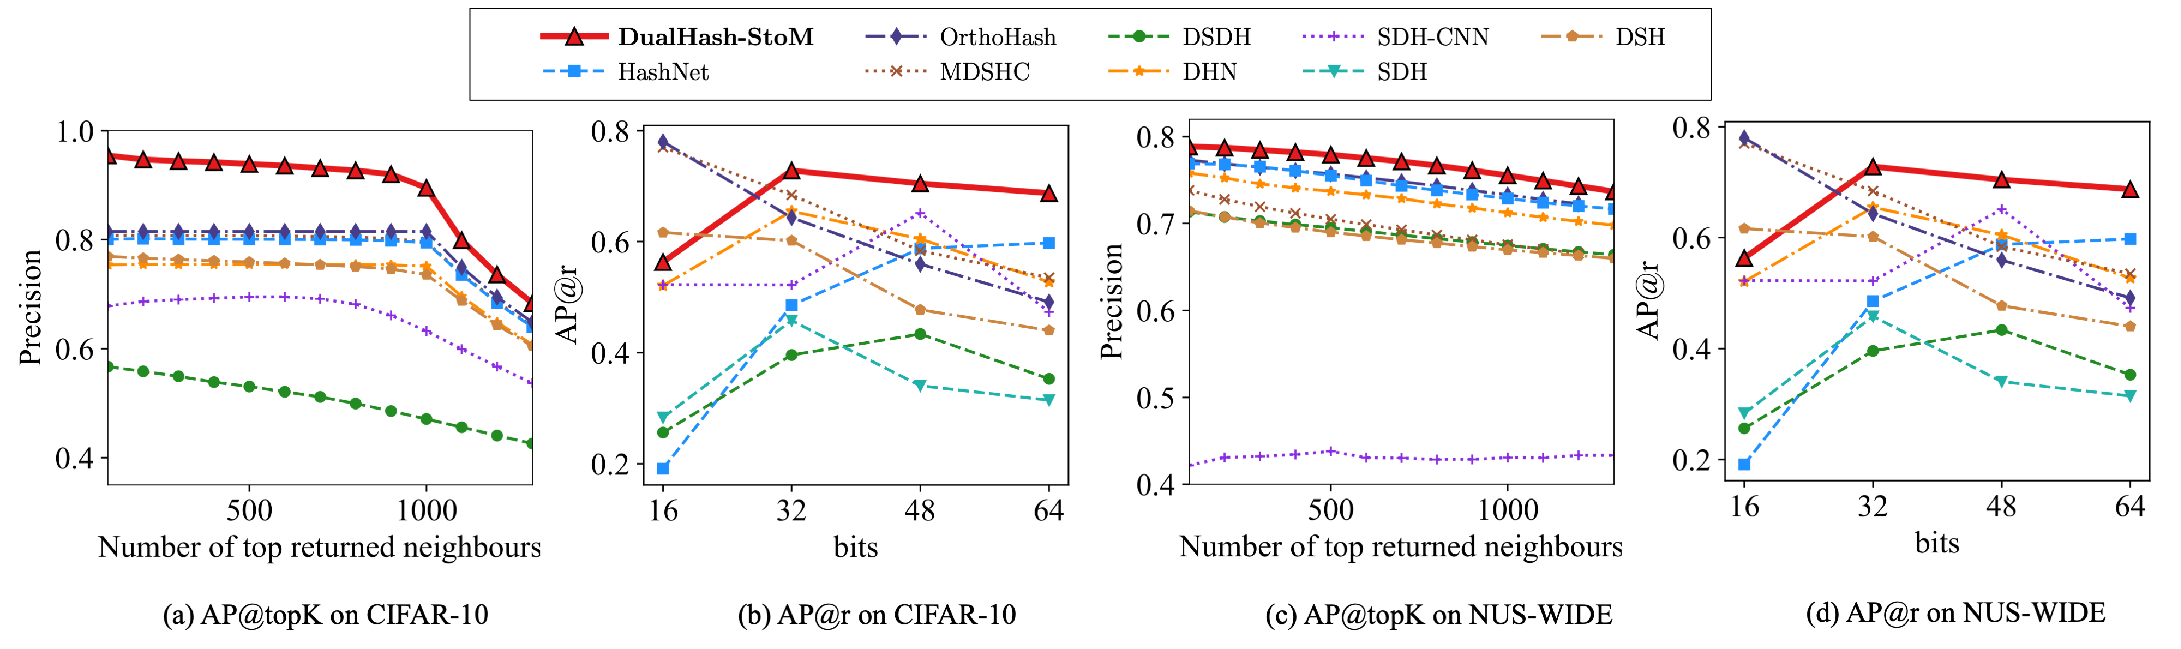
\includegraphics[width=0.98\textwidth,trim=0 4 523 53,clip]{results_images/ex2_4figures.pdf}
% \end{center}
% \vspace{-0.06cm}
% \begin{itemize}
% \item \blue{P@topK:} DualHash-StoM maintains the highest precision for the most relevant retrieved neighbours.
% \item \blue{P@r=2:} performance peaks at 32 bits and remains strong at longer code lengths.
% \end{itemize}
% \end{frame}


\begin{frame}{Retrieval Performance: NUS-WIDE}
\vspace{0.05cm}
\begin{center}
% Shared legend extracted from Figure 6.2.
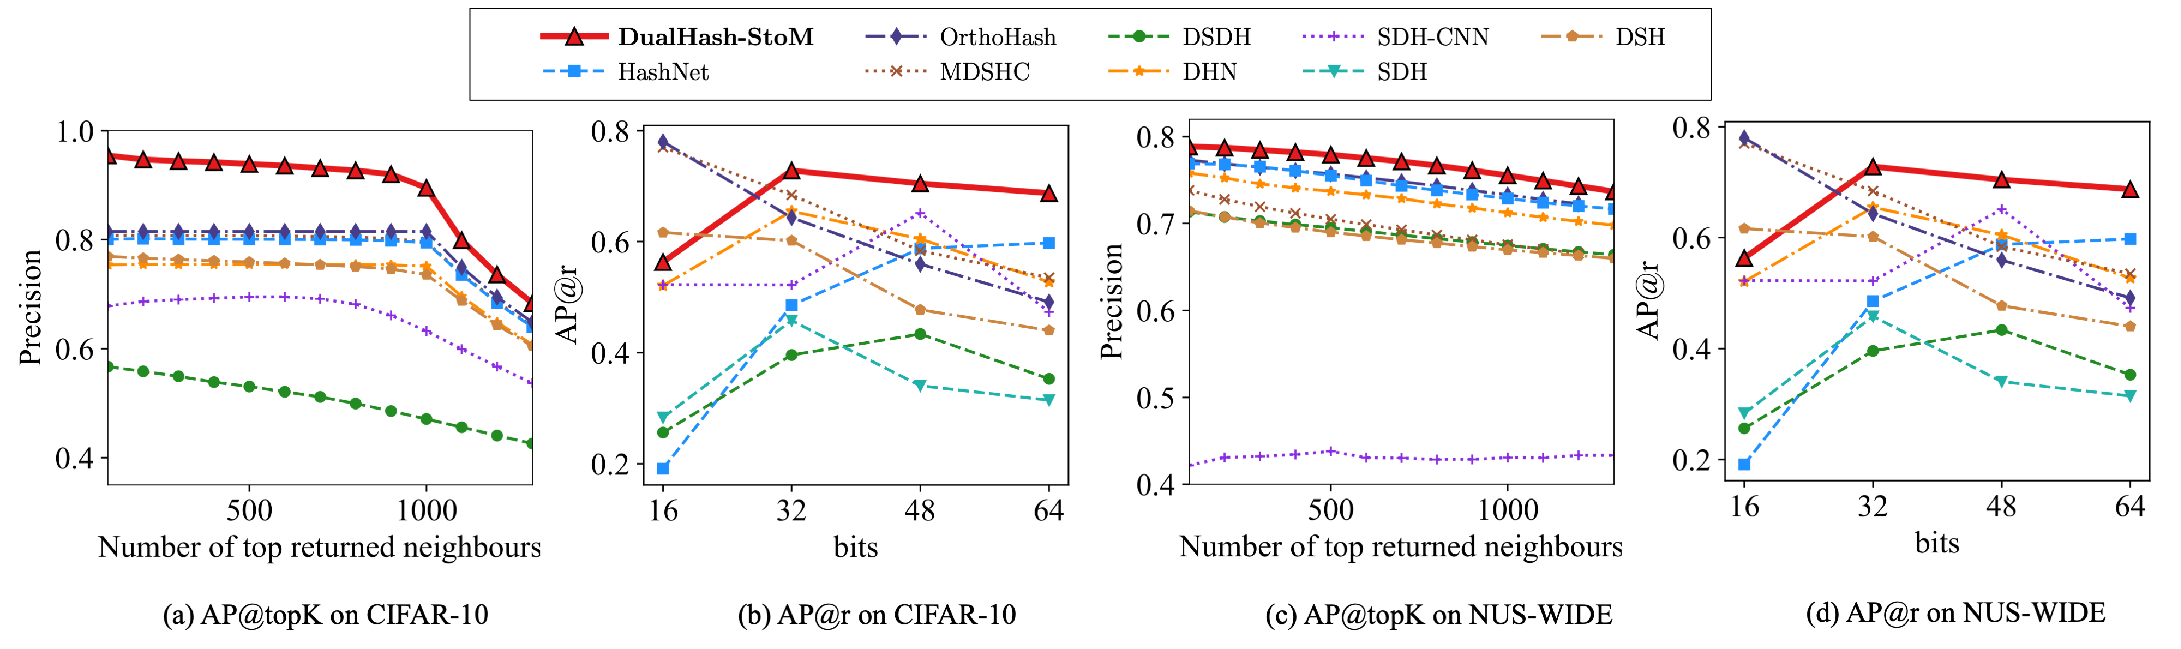
\includegraphics[width=0.76\textwidth,trim=200 264 200 0,clip]{results_images/ex2_4figures.pdf}
\\[-0.02cm]
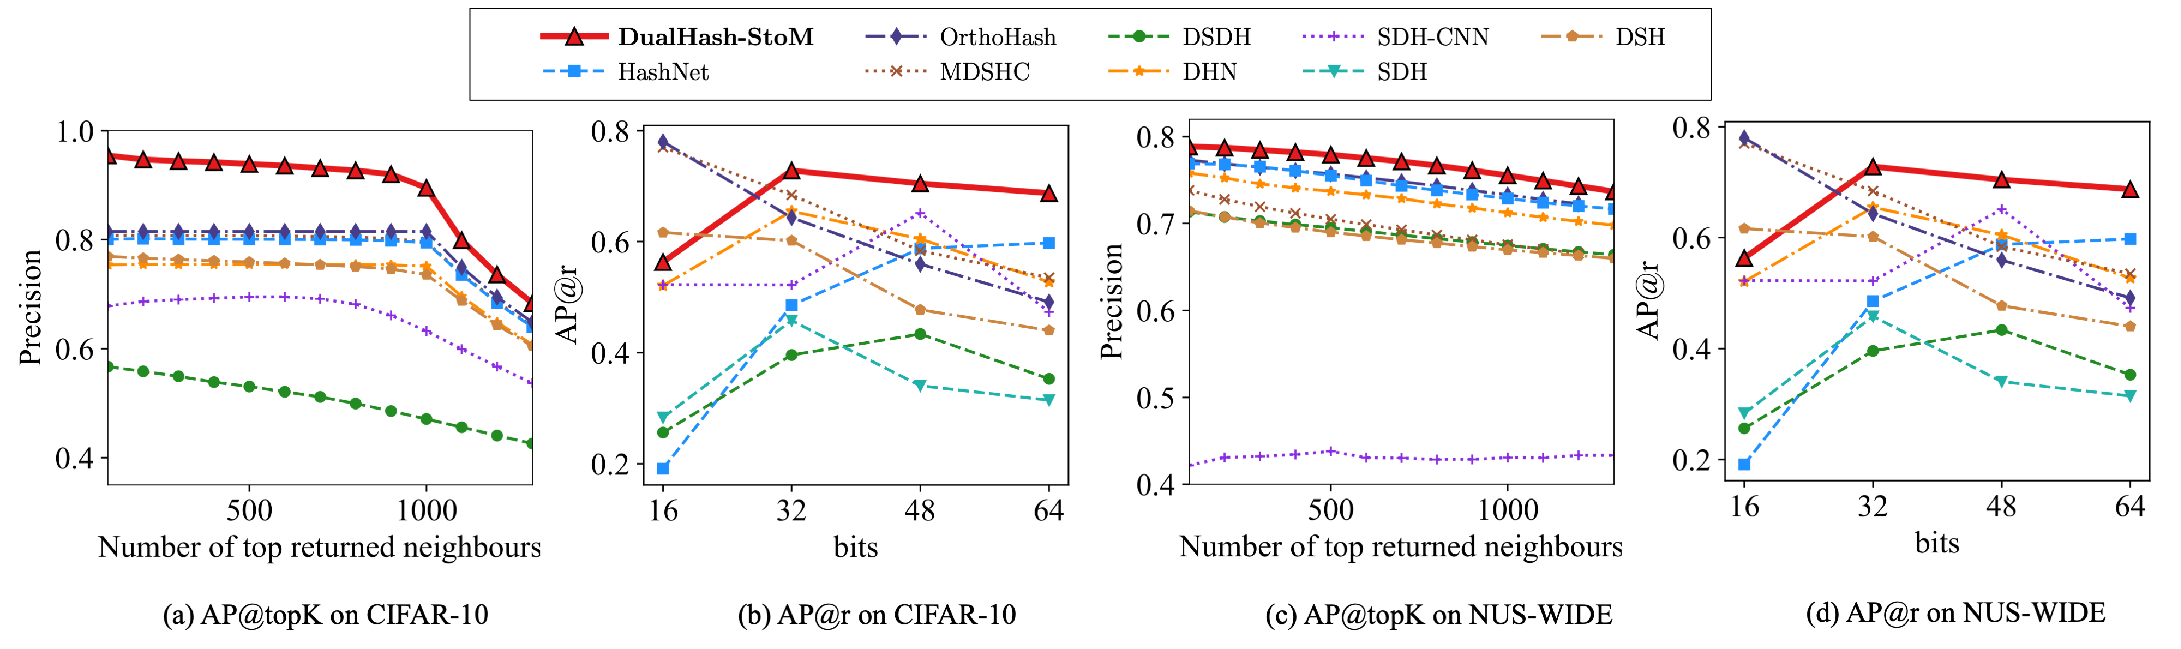
\includegraphics[width=0.98\textwidth,trim=523 4 0 53,clip]{results_images/ex2_4figures.pdf}
\end{center}
\vspace{-0.06cm}
\begin{itemize}
\item \blue{P@topK:} DualHash-StoM preserves the best precision across the top-ranked results.
\item \blue{P@r=2:} DualHash-StoM remains competitive across 32--64-bit codes on the multi-label dataset.
\end{itemize}
\end{frame}


\begin{frame}{Quantization Error Analysis}
\vspace{0.15cm}
\begin{columns}[T,onlytextwidth]
  \column{0.54\textwidth}
  \centering
  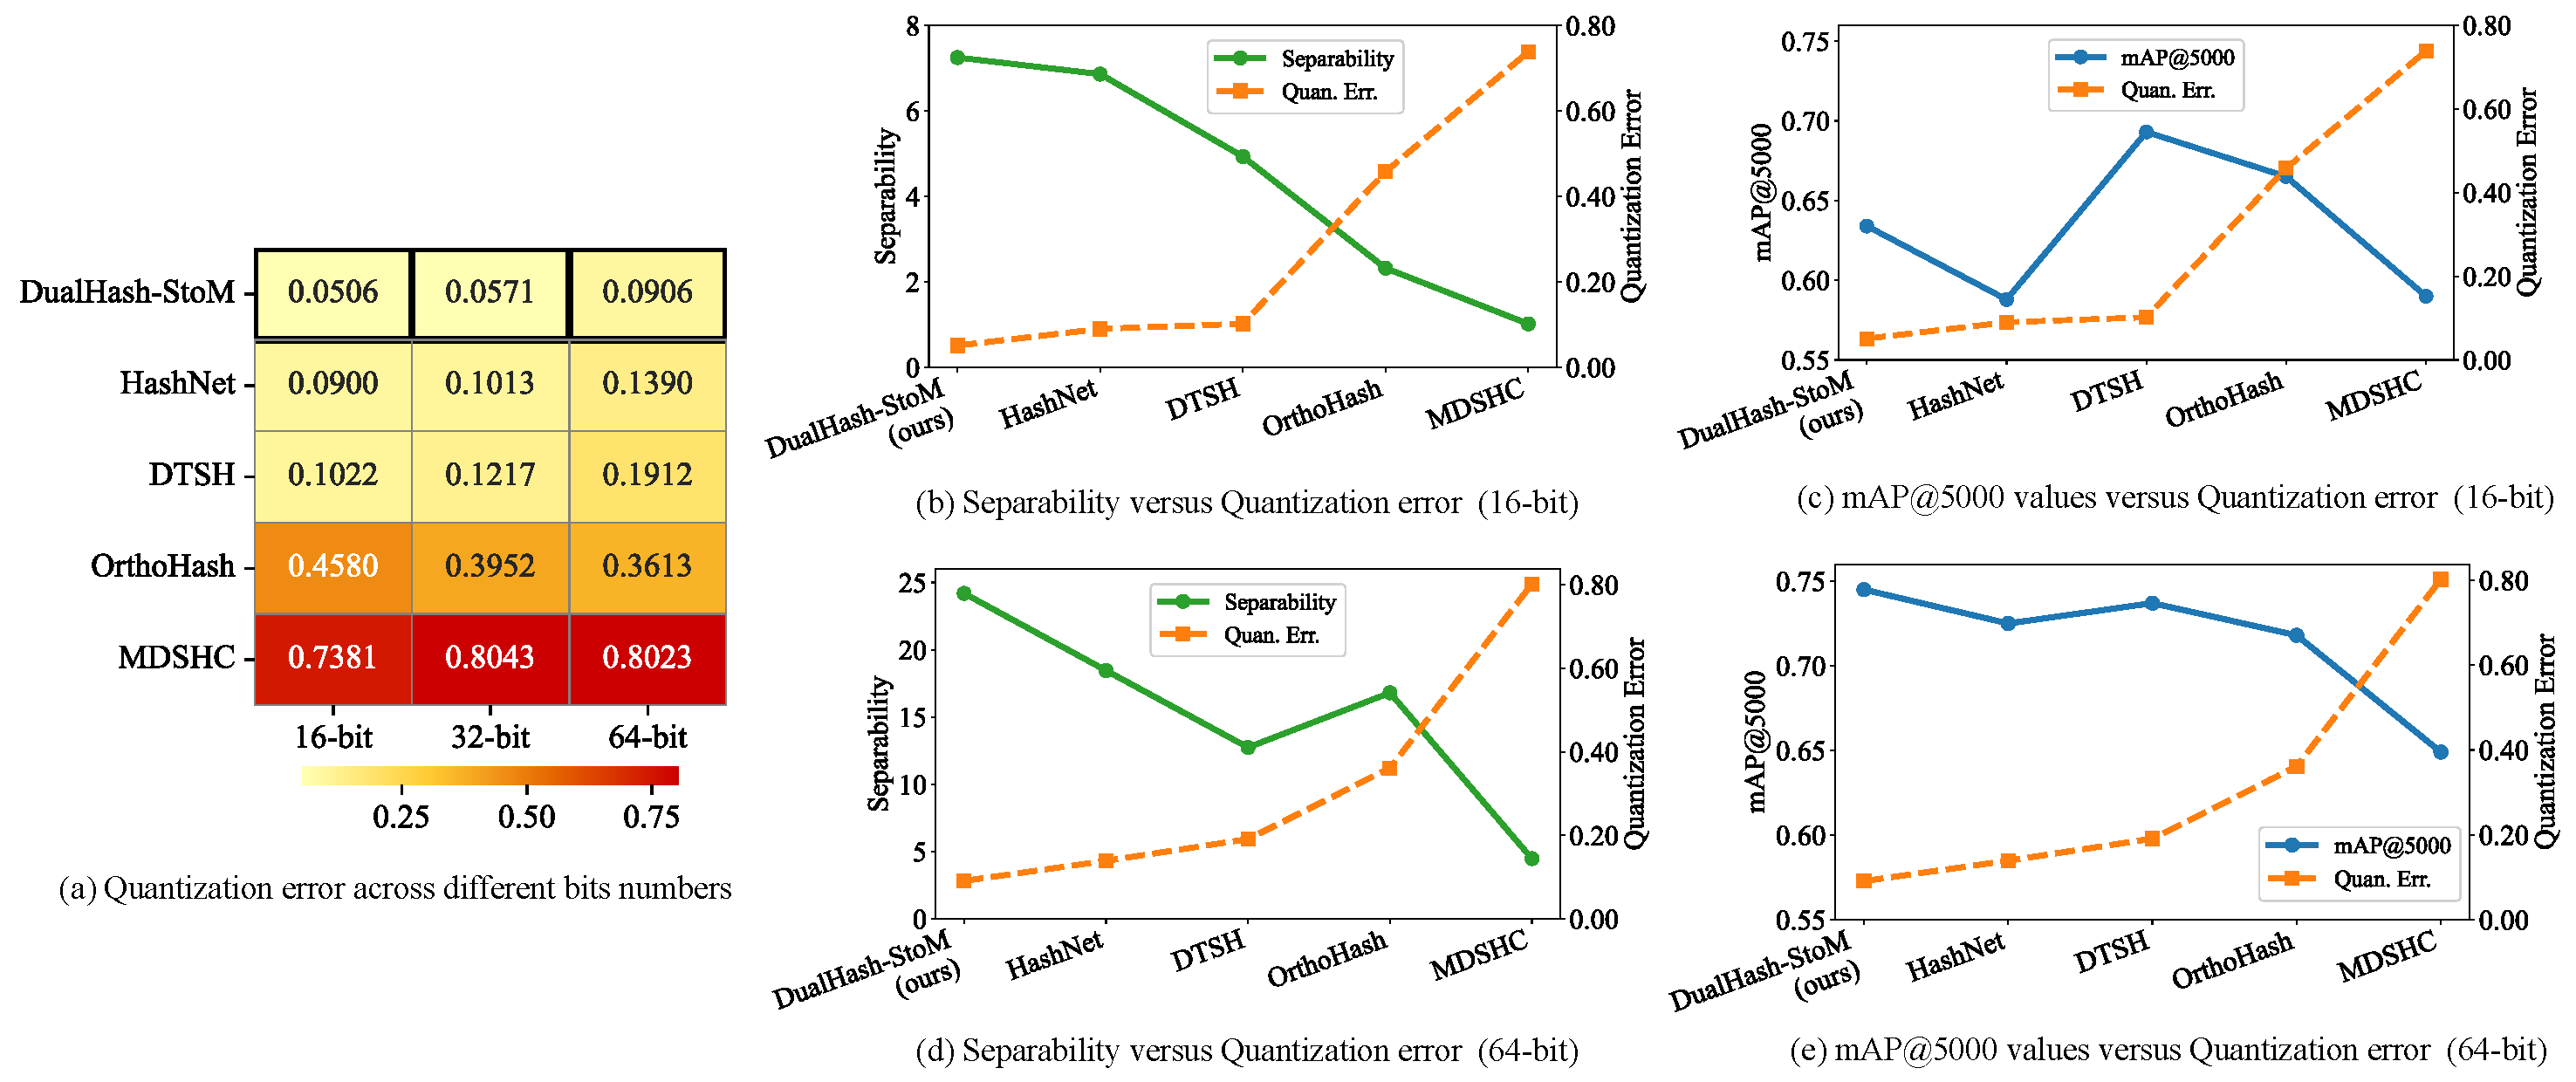
\includegraphics[width=\linewidth,height=0.68\textheight,keepaspectratio,
    trim=0 0 1000 0,clip]{results_images/quantization_error_further_analysis.pdf}
  \\
  \vspace{0.05cm}
  {\scriptsize Figure 6.3(a): Quantization error across bit lengths.}
% 大图
  \column{0.42\textwidth}
  \vspace{0.25cm}
  \begin{itemize}
  \item DualHash attains the \blue{smallest quantization error} across different bit lengths among all evaluated methods.
  \vspace{0.28cm}
  \item This stems from the \blue{dual-space reformulation}: convexity of $h^*$ yields optimization advantages over the nonconvex primal.
  \end{itemize}
\end{columns}
\end{frame}


% \begin{frame}{Parameter Sensitivity}
% \vspace{0.1cm}

% \begin{center}
% \includegraphics[width=0.88\textwidth,height=0.68\textheight,keepaspectratio]{results_images/sensitivity_2datasets.pdf}
% \end{center}

% \vspace{-0.1cm}
% \begin{itemize}
% \item DualHash-StoM is \blue{robust} across
% $\eta\in\{10^{-5},10^{-3},10^{-2},1\}$ and $\gamma\in\{0.3,3,30,100\}$.
% \item The 64-bit mAP variation is below $3\%$ on CIFAR-10 and below $8\%$ on NUS-WIDE.
% \end{itemize}
% \end{frame}


\section{Summary}
% \begin{frame}{Contributions}
% \vspace{0.3cm}

% \begin{itemize}
% \item[\blue{$\triangleright$}] \textbf{Novel primal-dual hashing algorithms.}
% We reformulate deep hashing with W-type regularization as a finite-sum multi-block optimization, decoupling the composite term $h(\bD(\bx))$ via Fenchel duality, yielding closed-form dual updates. Two instances: \textbf{DualHash-StoM} (momentum) and \textbf{DualHash-StoRM} (variance reduction).

% \vspace{0.25cm}
% \item[\blue{$\triangleright$}] \textbf{Comparable complexity guarantee.}
% $\calO(\varepsilon^{-4})$ for DualHash-StoM and $\calO(\varepsilon^{-3})$ for DualHash-StoRM under mean-squared smoothness, matching the best-known lower bound.

% \vspace{0.25cm}
% \item[\blue{$\triangleright$}] \textbf{Superior empirical performance.}
% Consistently lower quantization errors and higher retrieval accuracy on three datasets.
% \end{itemize}
% \end{frame}

\begin{frame}{Summary}
\vspace{0.2cm}

\begin{itemize}
\item[\blue{$\bullet$}] \textbf{DualHash:} a stochastic primal-dual algorithm for deep hashing via Fenchel duality.
\begin{itemize}
\item Handles \blue{nonsmooth W-type regularization} with nonlinear composition.
\item Closed-form dual proximal update bypasses the intractable $\prox_{h\circ\bD}$.
\item Oracle complexity:
\[
\text{DualHash-StoM:}\ \calO(\varepsilon^{-4}),\qquad
\text{DualHash-StoRM:}\ \calO(\varepsilon^{-3}).
\]
\end{itemize}
\end{itemize}

\vspace{0.2cm}
\begin{block}{Future work}
\begin{itemize}
% \item Extend the decoupling-dual-structure principle to quantization-aware training of low-bit neural networks.
\item Characterize the gap between stationary points of (P) and the original composite problem as penalty parameter $\gamma\to\infty$.
\end{itemize}
\end{block}

\vfill
{
\noindent\textsuperscript{1} Luxuan Li, Xiao Wang, and Chunfeng Cui. \emph{DualHash: A Stochastic Primal-Dual Algorithm with Theoretical Guarantee for Deep Hashing}. arXiv preprint \href{https://arxiv.org/abs/2510.18218}{arXiv:2510.18218}.}
\end{frame}


\begin{frame}[t]{Co-authors}
\small
\vspace{0.5cm}

\begin{columns}[T,onlytextwidth]
  \column{0.48\textwidth}
  \centering
  \begin{minipage}[c][3.2cm][c]{0.68\linewidth}
    \centering
    
\includegraphics[height=3.0cm,keepaspectratio]{figures/liluxuan.jpg}
  \end{minipage}

  \vspace{0.28cm}
  {\large Luxuan Li}\par
  \vspace{0.08cm}
  {\normalsize Third-year Ph.D. Student}\par
  \vspace{0.04cm}
  {\normalsize School of Mathematical Sciences}\par
  \vspace{0.04cm}
  {\normalsize Beihang University}\par

  \column{0.48\textwidth}
  \centering
  \begin{minipage}[c][3.2cm][c]{0.68\linewidth}
    \centering
    
\includegraphics[height=3.0cm,keepaspectratio]{figures/wangxiao.png}
  \end{minipage}

  \vspace{0.28cm}
  {\large Prof. Xiao Wang}\par
  \vspace{0.08cm}
  {\normalsize School of Computer Science and Engineering}\par
  \vspace{0.04cm}
  {\normalsize Sun Yat-Sen University}\par
\end{columns}
\end{frame}

\begin{frame}
\centering
\vfill
{\Huge\blue{Thank You!}}\\[0.45cm]
\vfill
\end{frame}


\begin{frame}[t]{References}
\begin{itemize}
\item[\textbf{[1]}] Chambolle A., Pock T. A first-order primal-dual algorithm for convex problems with applications to imaging. Journal of Mathematical Imaging and Vision, 2011, 40(1): 120--145.
\item[\textbf{[2]}] Bai Y. et al. ProxQuant: Quantized neural networks via proximal operators. ICLR, 2019.
\item[\textbf{[3]}] Davis D., Drusvyatskiy D. Stochastic model-based minimization of weakly convex functions. SIAM J. Optim., 2019, 29(1): 207--239.
\item[\textbf{[4]}] Bolte J. et al. Nonconvex Lagrangian-based optimization: Monitoring schemes and global convergence. Math. Oper. Res., 2018, 43(4): 1210--1232.
\item[\textbf{[5]}] Zhu D. et al. A first-order primal-dual method for nonconvex constrained optimization based on the augmented Lagrangian. Math. Oper. Res., 2024, 49(1): 125--150.
\item[\textbf{[6]}] Chen X. et al. Convergence of three-block ADMM for weakly convex optimization problems. SIAM J. Imaging Sci., 2025, 18(1): 449--493.
\item[\textbf{[7]}] Yao Y. et al. A note on complexity for two classes of structured non-smooth non-convex compositional optimization. arXiv:2411.14342, 2024.
\end{itemize}
\end{frame}

\begin{frame}[t]{References}
\begin{itemize}
\item[\textbf{[8]}] Zhang H. et al. Complexity and convergence analysis of a single-loop SDCAM for Lipschitz composite optimization and beyond. arXiv:2512.24059, 2025.
\item[\textbf{[9]}] Shen F. et al. Supervised discrete hashing. CVPR, 2015: 37--45.
\item[\textbf{[10]}] Zhu H. et al. Deep hashing network for efficient similarity retrieval. AAAI, 2016: 2415--2421.
\item[\textbf{[11]}] Wang L. et al. Deep hashing with minimal-distance-separated hash centers. CVPR, 2023: 23455--23464.
\item[\textbf{[12]}] Guo J. Preconditioned primal--dual gradient methods for nonconvex composite and finite-sum optimization. AIMS Mathematics, 2026, 11(1): 2188--2226.
\item[\textbf{[13]}] Hertrich J., Steidl G. Inertial stochastic PALM and applications in machine learning. Sampling Theory, Signal Processing, and Data Analysis, 2022, 20(1): Article 4.
\item[\textbf{[14]}] Jiang B., Lin T., Ma S., Zhang S. Structured nonconvex and nonsmooth optimization: Algorithms and iteration complexity analysis. Computational Optimization and Applications, 2019, 72(1): 115--157.
\end{itemize}
\end{frame}


\end{document}
